\chapter{二项堆、斐波那契堆、贪心}

\section{回顾}
上一节我们从探究贪心和动态规划的关系,从最短路的动态规划算法转到了Dijstra算法,原先只是要求没有负圈,可以做动态规划。如果进一步加强条件,要求没有负的边,可以做Dijstra算法。 \\
而关于Dijstra算法,其数据结构非常重要,尤其斐波那契堆这种数据结构是专门为Dijstra算法发明出来的。关于斐波那契堆还有一方面是其采用了均摊分析的方法。

首先来看下做这个数据结构的时候,最基本的出发点是什么。总体来说我们是要做一个优先队列,因为我们在Dijstra算法中,总是要在集合中找最小数。优先队列可以理解为,在队列中一个数越小就应该放在前面,所以实现这种数据结构,我们最直观简单的是开辟一个数组,但是存在一些问题,比如从N个数中找最小可能需

要从头到尾找一遍,即使预先做好排序,在插入时也会非常耗时。所以基于这些问题,提出了二叉堆。从数组到二叉堆的转变,对于原先严格的排序现在放松要求,二叉堆中不要求完全n个数有序,只要部分有序即可,只要一个节点比其儿子节点小就行,称为堆序。但是两个堆在合并时又比较麻烦,我们继续做思路上的转变,可以继续放松要求,不一定非得一棵树,如果可以有多棵数,两个堆的合并直接放一起就行。\\
基本思想:可以放松,但是不要太多,可以有多棵数,树的数目不要太多。

\section{二项堆}
树的数目不能太多,因为我们毕竟要找所有树中最小的数,每棵树最小都在根节点,就直接把每个树的根节点比较下,显然如果有n棵树的话,就和数组没啥区别,所以要限制数的数目。图示为两个堆树。
\begin{figure}[h!]
\centering
\begin{tikzpicture}[scale=0.9, auto,swap]

    \foreach \pos/\name/\label in {{(0,0)/root/21}, {(-1,-1)/L/25}, {(1,-1)/R/27}, {(-1.5,-2)/LL/29}}
        \node[middlevertex,draw=black, fill=white!20] (\name) at \pos {\tiny $\label$};
    \foreach \source/ \dest /\weight in {root/L/{}, root/R/{}, L/LL/{}}
        \path[undirectededge] (\source) -- node[weight] {$\weight$} (\dest);
        
 \node[ultra thick, above, blue] at (root.north)  {$H_1$}; 

    \foreach \pos/\name/\label in {{(4+0,0)/root/6}, {(4-1,-1)/L/8}, {(4+1,-1)/R/11}}
        \node[middlevertex,draw=black, fill=white!20] (\name) at \pos {\tiny $\label$};
    \foreach \source/ \dest /\weight in {root/L/{}, root/R/{}}
        \path[undirectededge] (\source) -- node[weight] {$\weight$} (\dest);
 \node[ultra thick, above, blue] at (root.north)  {$H_2$};  		
\end{tikzpicture}
\end{figure} 

\subsection{如何控制数的数目:合并树}
为了控制数的数目不能太多,加了一个合并的操作。如图所示,每次合并时找同等级的树,合并的规则和堆合并的规则一样,合并完父节点的数比子节点的数都要小,下图分别为一级的数和二级的树的合并操作。



\begin{figure}[!htbp]
\centering
\begin{tikzpicture}[scale=0.9, auto,swap]

   \def\dx{0};
   \def\dy{1.5};
    \foreach \pos/\name/\label in {{(0 +\dx,0 +\dy)/root/6}, {(1.5 + \dx, 0 + \dy)/L/11}} 
            \node[middlevertex,draw=black, fill=white!20] (\name) at \pos {\tiny $\label$};
   	


   \draw[->, line width=2pt, blue] (2, 2-0.5) -- node[above]{$link$} (3, 2-0.5); 
   \def\dx{3.5};
   \def\dy{2};
    \foreach \pos/\name/\label in {{(0 +\dx,0 +\dy)/root/6}, {(0 + \dx, -1 + \dy)/L/11}} 
            \node[middlevertex,draw=black, fill=white!20] (\name) at \pos {\tiny $\label$};
    \foreach \source/ \dest /\weight in {root/L/{}}
        \path[undirectededge] (\source) -- node[weight] {$\weight$} (\dest);


   \def\dx{0};
   \def\dy{0};
    \foreach \pos/\name/\label in {{(0 +\dx,0 +\dy)/root/6}, {(0 + \dx, -1 + \dy)/L/11}} 
            \node[middlevertex,draw=black, fill=white!20] (\name) at \pos {\tiny $\label$};
    \foreach \source/ \dest /\weight in {root/L/{}}
        \path[undirectededge] (\source) -- node[weight] {$\weight$} (\dest);


   \def\dx{1.5};
   \def\dy{0};
    \foreach \pos/\name/\label in {{(0 +\dx,0 +\dy)/root/8}, {(0 + \dx, -1 + \dy)/L/9}} 
            \node[middlevertex,draw=black, fill=white!20] (\name) at \pos {\tiny $\label$};
    \foreach \source/ \dest /\weight in {root/L/{}}
        \path[undirectededge] (\source) -- node[weight] {$\weight$} (\dest);

   \draw[->, line width=2pt, blue] (2, -0.5) -- node[above]{$link$} (3, -0.5); 
   

   \def\dx{3.5};
   \def\dy{0};
    \foreach \pos/\name/\label in {{(0 +\dx,0 +\dy)/root/6}, {(0 + \dx, -1 + \dy)/L/11}} 
            \node[middlevertex,draw=black, fill=white!20] (\name) at \pos {\tiny $\label$};
    \foreach \source/ \dest /\weight in {root/L/{}}
        \path[undirectededge] (\source) -- node[weight] {$\weight$} (\dest);

   \def\dx{4.5};
   \def\dy{-1};
    \foreach \pos/\name/\label in {{(0 +\dx,0 +\dy)/R/8}, {(0 + \dx, -1 + \dy)/RL/9}} 
            \node[middlevertex,draw=black, fill=white!20] (\name) at \pos {\tiny $\label$};
    \foreach \source/ \dest /\weight in {R/RL/{}, root/R/{}}
        \path[undirectededge] (\source) -- node[weight] {$\weight$} (\dest);
   \end{tikzpicture}
\end{figure} 

\subsection{二项树及其性质}
二项树是一个递归的定义,只有一个节点的为$B_0$,两个$B_k$等级的堆树合并为一个等级为$B_{k+1}$的堆树。如图:
\begin{figure}[!htbp]
\centering
\begin{tikzpicture}[scale=1., auto,swap]

  \def\dx{0};
  \def\dy{0}; 
  
   \draw[thick, fill=green!20] (0, 0) -- (-0.5, -0.73) -- (0.5, -0.73) -- (0,0); 
   \node[ thick, blue] at (0, -0.48) { $B_k$};
   \draw[thick, fill=green!20] (1.5+0, 0-1) -- (1.5-0.5, -0.73-1) -- (1.5+0.5, -0.73-1) -- (1.5+0,0-1); 
   \node[ thick, blue] at (0+1.5, -0.48-1) {$B_k$};
 
   \foreach \x/\y/\name/\label in { 0/0/root/, 1.5/-1/L11/}
          \node[tinyvertex,draw=black, fill=white!20] (\name) at (\x+\dx, \y + \dy) {\tiny $\label$};
  
   \node[ thick, blue, above ] at (root.north) { $B_{k+1}$};
 
 
  \foreach \source/ \dest /\weight in {root/L11/{}}
         \path[undirectededge] (\source) -- node[weight] {$\weight$} (\dest);
 
   \foreach \x/\y/\name/\label in { -2/0/root/}
          \node[tinyvertex,draw=black, fill=white!20] (\name) at (\x+\dx, \y + \dy) {\tiny $\label$};

   \node[ thick, blue, above ] at (root.north) { $B_{0}$};
  
   \end{tikzpicture}
\end{figure} \\
我们通过一些直观的例子来理解下二项树
\begin{figure}[!htbp]
\centering
\begin{tikzpicture}[scale=1., auto,swap]

  \def\dx{0};
  \def\dy{0}; 
 \def\u{0.8};
  
   \foreach \x/\y/\name/\label in { 0/0/root/6}
          \node[smallvertex,draw=black, fill=white!20] (\name) at (\x*\u+\dx, \y + \dy) {\tiny $\label$};
  
  \node[above, blue, ultra thick] at (root.north) {$B_0$};
  
   \end{tikzpicture}
\end{figure}


\begin{figure}[!htbp]
\centering
\begin{tikzpicture}[scale=1., auto,swap]

  \def\dx{0};
  \def\dy{0}; 
 \def\u{0.8};
  
   \foreach \x/\y/\name/\label in { 0/0/root/6, 0/-1/L11/8}
          \node[smallvertex,draw=black, fill=white!20] (\name) at (\x*\u+\dx, \y + \dy) {\tiny $\label$};
  
  \foreach \source/ \dest /\weight in {root/L11/{}}
         \path[undirectededge] (\source) -- node[weight] {$\weight$} (\dest);
 
  \node[above, blue, ultra thick] at (root.north) {$B_1$};
  
   \end{tikzpicture}
\end{figure}


\begin{figure}[!htbp]
\centering
\begin{tikzpicture}[scale=1., auto,swap]

  \def\dx{0};
  \def\dy{0}; 
 \def\u{0.8};
  
   \foreach \x/\y/\name/\label in { 0/0/root/6, 0/-1/L11/8, 1/-1/L12/9, 1/-2/L21/10}
          \node[smallvertex,draw=black, fill=white!20] (\name) at (\x*\u+\dx, \y + \dy) {\tiny $\label$};
  

  
  \foreach \source/ \dest /\weight in {root/L11/{}, root/L12/{}}
         \path[undirectededge] (\source) -- node[weight] {$\weight$} (\dest);
 
 

  \foreach \source/ \dest /\weight in {L12/L21/{}}
         \path[undirectededge] (\source) -- node[weight] {$\weight$} (\dest);
 
  \node[above, blue, ultra thick] at (root.north) {$B_2$};
  
   \end{tikzpicture}
\end{figure}
存在以下性质:(1)每棵树$B_k$的节点个数为$2^k$ (2)树的高度为k。(3)从左往右儿子分别分$B_0,B_1,B_2 ... B_k$,非常规则的一棵树
可以观察到:对于每颗数每层的个数存在以下规则\\
\begin{center}
$B_0:1$ \\
$B_1:1 1$ \\
$B_2:1 2 1$\\
$B_3:1 3 3 1$ \\
$B_4:1 4 6 4 1$ \\
\end{center}
刚好为二项式的系数,所以将这种结构称为二项树。那么我们一直强调控制树的个数,只要存在等级相同的树将其合并,那么最终形成的森林里,每个等级的数只有一个,如图例子中,$B_0,B_1,B_2,B_3$各有一棵。\\
\begin{figure}[!htbp]
\centering
\begin{tikzpicture}[scale=1., auto,swap]



 \draw[thick, dashed, blue] (0,0) -- (4,0);
 %B0
  \def\dx{0};
  \def\dy{0}; 
 \def\u{0.8};
  
   \foreach \x/\y/\name/\label in { 0/0/root/3}
          \node[smallvertex,draw=black, fill=white!20] (\name) at (\x*\u+\dx, \y + \dy) {\tiny $\label$};
    
   \node[ultra thick, blue, above] at (root.north) {$B_0$};  

  %B1
  \def\dx{1};
  \def\dy{0}; 
 \def\u{0.8};
  
   \foreach \x/\y/\name/\label in { 0/0/root/4, 0/-1/L11/8}
          \node[smallvertex,draw=black, fill=white!20] (\name) at (\x*\u+\dx, \y + \dy) {\tiny $\label$};
  

  
  \foreach \source/ \dest /\weight in {root/L11/{}}
         \path[undirectededge] (\source) -- node[weight] {$\weight$} (\dest);
 

 \node[ultra thick, blue, above] at (root.north) {$B_1$};  

%B2
  \def\dx{2};
  \def\dy{0}; 
 \def\u{0.8};
  
   \foreach \x/\y/\name/\label in { 0/0/root/5, 0/-1/L11/8, 1/-1/L12/9, 1/-2/L21/10}
          \node[smallvertex,draw=black, fill=white!20] (\name) at (\x*\u+\dx, \y + \dy) {\tiny $\label$};
  

  
  \foreach \source/ \dest /\weight in {root/L11/{}, root/L12/{}}
         \path[undirectededge] (\source) -- node[weight] {$\weight$} (\dest);
 
 

  \foreach \source/ \dest /\weight in {L12/L21/{}}
         \path[undirectededge] (\source) -- node[weight] {$\weight$} (\dest);
 
   \node[ultra thick, blue, above] at (root.north) {$B_2$};  

  %B3

  \def\dx{4};
  \def\dy{0}; 
 \def\u{0.8};
  
   \foreach \x/\y/\name/\label in { 0/0/root/6, 0/-1/L11/8, 1/-1/L12/9, 2/-1/L13/7} 
          \node[smallvertex,draw=black, fill=white!20] (\name) at (\x*\u+\dx, \y + \dy) {\tiny $\label$};
  
   \foreach \x/\y/\name/\label in {1/-2/L21/10, 2/-2/L22/11/, 3/-2/L23/12}
          \node[smallvertex,draw=black, fill=white!20] (\name) at (\x*\u+\dx, \y + \dy) {\tiny $\label$};

   \foreach \x/\y/\name/\label in {3/-3/L31/14}
          \node[smallvertex,draw=black, fill=white!20] (\name) at (\x*\u+\dx, \y + \dy) {\tiny $\label$};

  
  \foreach \source/ \dest /\weight in {root/L11/{}, root/L12/{}, root/L13/{}}
         \path[undirectededge] (\source) -- node[weight] {$\weight$} (\dest);
 
  \foreach \source/ \dest /\weight in {L12/L21/{}, L13/L22/{}, L13/L23/{}, L23/L31/{}}
         \path[undirectededge] (\source) -- node[weight] {$\weight$} (\dest);
 
 \node[ultra thick, blue, above] at (root.north) {$B_3$};  

   \end{tikzpicture}
\end{figure}
我们对两个堆树合并时只需要简单把两个堆树加起来,但是对于下图的例子,加起来有两个$B_1$,按照我们的规则最多只能有一个等级的树。就需要把两个$B_1$合并成一棵$B_2$,合并完之后又出现两棵$B_2$,再次合并两棵$B_2$成$B_3$,以此最终合成一棵$B_4$。

\begin{figure}[!htbp]
\centering
\begin{tikzpicture}[scale=0.9, auto,swap]

 \draw[thick, dashed, blue] (1,0) -- (2,0);

 \draw[thick, dashed, blue] (4,0) -- (6,0);

\node[ultra thick, red] at (3.5, -0.5) {\Large $+$};

  %B1
  \def\dx{1};
  \def\dy{0}; 
 \def\u{0.8};
  
   \foreach \x/\y/\name/\label in { 0/0/root/3, 0/-1/L11/7}
          \node[smallvertex,draw=black, fill=white!20] (\name) at (\x*\u+\dx, \y + \dy) {\tiny $\label$};
  

  
  \foreach \source/ \dest /\weight in {root/L11/{}}
         \path[undirectededge] (\source) -- node[weight] {$\weight$} (\dest);

  \node[ultra thick, blue, above] at (root.north) {$B_1$};  
    
  %B1
  \def\dx{4};
  \def\dy{0}; 
 \def\u{0.8};
  
   \foreach \x/\y/\name/\label in { 0/0/root/4, 0/-1/L11/8}
          \node[smallvertex,draw=black, fill=white!20] (\name) at (\x*\u+\dx, \y + \dy) {\tiny $\label$};
  

  
  \foreach \source/ \dest /\weight in {root/L11/{}}
         \path[undirectededge] (\source) -- node[weight] {$\weight$} (\dest);
 

  \node[ultra thick, blue, above] at (root.north) {$B_1$};  

%B2
  \def\dx{2};
  \def\dy{0}; 
 \def\u{0.8};
  
   \foreach \x/\y/\name/\label in { 0/0/root/5, 0/-1/L11/8, 1/-1/L12/9, 1/-2/L21/10}
          \node[smallvertex,draw=black, fill=white!20] (\name) at (\x*\u+\dx, \y + \dy) {\tiny $\label$};
  

  
  \foreach \source/ \dest /\weight in {root/L11/{}, root/L12/{}}
         \path[undirectededge] (\source) -- node[weight] {$\weight$} (\dest);
 
 

  \foreach \source/ \dest /\weight in {L12/L21/{}}
         \path[undirectededge] (\source) -- node[weight] {$\weight$} (\dest);
 
    \node[ultra thick, blue, above] at (root.north) {$B_2$};  

  %B3

  \def\dx{6};
  \def\dy{0}; 
 \def\u{0.8};
  
   \foreach \x/\y/\name/\label in { 0/0/root/6, 0/-1/L11/8, 1/-1/L12/9, 2/-1/L13/7} 
          \node[smallvertex,draw=black, fill=white!20] (\name) at (\x*\u+\dx, \y + \dy) {\tiny $\label$};
  
   \foreach \x/\y/\name/\label in {1/-2/L21/10, 2/-2/L22/11/, 3/-2/L23/12}
          \node[smallvertex,draw=black, fill=white!20] (\name) at (\x*\u+\dx, \y + \dy) {\tiny $\label$};

   \foreach \x/\y/\name/\label in {3/-3/L31/14}
          \node[smallvertex,draw=black, fill=white!20] (\name) at (\x*\u+\dx, \y + \dy) {\tiny $\label$};

  
  \foreach \source/ \dest /\weight in {root/L11/{}, root/L12/{}, root/L13/{}}
         \path[undirectededge] (\source) -- node[weight] {$\weight$} (\dest);
 
  \foreach \source/ \dest /\weight in {L12/L21/{}, L13/L22/{}, L13/L23/{}, L23/L31/{}}
         \path[undirectededge] (\source) -- node[weight] {$\weight$} (\dest);
 
  \node[ultra thick, blue, above] at (root.north) {$B_3$};  








 \draw[thick, dashed, blue] (0,-3) -- (4,-3);

\node[ultra thick, red] at (-0.5, -3) {\Large $=$};
 \draw[thick, ] (0,-3) -- (1,-4);


  %B1
  \def\dx{0};
  \def\dy{-3}; 
 \def\u{0.8};
  
   \foreach \x/\y/\name/\label in { 0/0/root/3, 0/-1/L11/7}
          \node[smallvertex,draw=black, fill=white!20] (\name) at (\x*\u+\dx, \y + \dy) {\tiny $\label$};
  

  
  \foreach \source/ \dest /\weight in {root/L11/{}}
         \path[undirectededge] (\source) -- node[weight] {$\weight$} (\dest);
   
     \node[ultra thick, blue, above] at (root.north) {$B_2$};  
 
  %B1
  \def\dx{1};
  \def\dy{-4}; 
 \def\u{0.8};
  
   \foreach \x/\y/\name/\label in { 0/0/root/4, 0/-1/L11/8}
          \node[smallvertex,draw=black, fill=white!20] (\name) at (\x*\u+\dx, \y + \dy) {\tiny $\label$};
  

  
  \foreach \source/ \dest /\weight in {root/L11/{}}
         \path[undirectededge] (\source) -- node[weight] {$\weight$} (\dest);
 
 

%B2
  \def\dx{2};
  \def\dy{-3}; 
 \def\u{0.8};
  
   \foreach \x/\y/\name/\label in { 0/0/root/5, 0/-1/L11/8, 1/-1/L12/9, 1/-2/L21/10}
          \node[smallvertex,draw=black, fill=white!20] (\name) at (\x*\u+\dx, \y + \dy) {\tiny $\label$};
  

  
  \foreach \source/ \dest /\weight in {root/L11/{}, root/L12/{}}
         \path[undirectededge] (\source) -- node[weight] {$\weight$} (\dest);
 
 

  \foreach \source/ \dest /\weight in {L12/L21/{}}
         \path[undirectededge] (\source) -- node[weight] {$\weight$} (\dest);
 
 
  \node[ultra thick, blue, above] at (root.north) {$B_2$};  
 
  %B3

  \def\dx{4};
  \def\dy{-3}; 
 \def\u{0.8};
  
   \foreach \x/\y/\name/\label in { 0/0/root/6, 0/-1/L11/8, 1/-1/L12/9, 2/-1/L13/7} 
          \node[smallvertex,draw=black, fill=white!20] (\name) at (\x*\u+\dx, \y + \dy) {\tiny $\label$};
  
   \foreach \x/\y/\name/\label in {1/-2/L21/10, 2/-2/L22/11/, 3/-2/L23/12}
          \node[smallvertex,draw=black, fill=white!20] (\name) at (\x*\u+\dx, \y + \dy) {\tiny $\label$};

   \foreach \x/\y/\name/\label in {3/-3/L31/14}
          \node[smallvertex,draw=black, fill=white!20] (\name) at (\x*\u+\dx, \y + \dy) {\tiny $\label$};

  
  \foreach \source/ \dest /\weight in {root/L11/{}, root/L12/{}, root/L13/{}}
         \path[undirectededge] (\source) -- node[weight] {$\weight$} (\dest);
 
  \foreach \source/ \dest /\weight in {L12/L21/{}, L13/L22/{}, L13/L23/{}, L23/L31/{}}
         \path[undirectededge] (\source) -- node[weight] {$\weight$} (\dest);
 
 \node[ultra thick, blue, above] at (root.north) {$B_3$};    
   \end{tikzpicture}
\caption{ Consolidating two $B_1$ trees into a $B_2$ tree}
\end{figure}

\begin{figure}[!htbp]
\centering
\begin{tikzpicture}[scale=0.9, auto,swap]



 \draw[thick, dashed, blue] (1,0) -- (2,0);

 \draw[thick, dashed, blue] (4,0) -- (6,0);

\node[ultra thick, red] at (3.5, -0.5) {\Large $+$};

  %B1
  \def\dx{1};
  \def\dy{0}; 
 \def\u{0.8};
  
   \foreach \x/\y/\name/\label in { 0/0/root/3, 0/-1/L11/7}
          \node[smallvertex,draw=black, fill=white!20] (\name) at (\x*\u+\dx, \y + \dy) {\tiny $\label$};
  

  
  \foreach \source/ \dest /\weight in {root/L11/{}}
         \path[undirectededge] (\source) -- node[weight] {$\weight$} (\dest);
   
    \node[ultra thick, blue, above] at (root.north) {$B_1$};  
 
  %B1
  \def\dx{4};
  \def\dy{0}; 
 \def\u{0.8};
  
   \foreach \x/\y/\name/\label in { 0/0/root/4, 0/-1/L11/8}
          \node[smallvertex,draw=black, fill=white!20] (\name) at (\x*\u+\dx, \y + \dy) {\tiny $\label$};
  

  
  \foreach \source/ \dest /\weight in {root/L11/{}}
         \path[undirectededge] (\source) -- node[weight] {$\weight$} (\dest);
 
 \node[ultra thick, blue, above] at (root.north) {$B_1$};  

%B2
  \def\dx{2};
  \def\dy{0}; 
 \def\u{0.8};
  
   \foreach \x/\y/\name/\label in { 0/0/root/5, 0/-1/L11/8, 1/-1/L12/9, 1/-2/L21/10}
          \node[smallvertex,draw=black, fill=white!20] (\name) at (\x*\u+\dx, \y + \dy) {\tiny $\label$};
  

  
  \foreach \source/ \dest /\weight in {root/L11/{}, root/L12/{}}
         \path[undirectededge] (\source) -- node[weight] {$\weight$} (\dest);
 
 

  \foreach \source/ \dest /\weight in {L12/L21/{}}
         \path[undirectededge] (\source) -- node[weight] {$\weight$} (\dest);
 
   \node[ultra thick, blue, above] at (root.north) {$B_2$};  

  %B3

  \def\dx{6};
  \def\dy{0}; 
 \def\u{0.8};
  
   \foreach \x/\y/\name/\label in { 0/0/root/6, 0/-1/L11/8, 1/-1/L12/9, 2/-1/L13/7} 
          \node[smallvertex,draw=black, fill=white!20] (\name) at (\x*\u+\dx, \y + \dy) {\tiny $\label$};
  
   \foreach \x/\y/\name/\label in {1/-2/L21/10, 2/-2/L22/11/, 3/-2/L23/12}
          \node[smallvertex,draw=black, fill=white!20] (\name) at (\x*\u+\dx, \y + \dy) {\tiny $\label$};

   \foreach \x/\y/\name/\label in {3/-3/L31/14}
          \node[smallvertex,draw=black, fill=white!20] (\name) at (\x*\u+\dx, \y + \dy) {\tiny $\label$};

  
  \foreach \source/ \dest /\weight in {root/L11/{}, root/L12/{}, root/L13/{}}
         \path[undirectededge] (\source) -- node[weight] {$\weight$} (\dest);
 
  \foreach \source/ \dest /\weight in {L12/L21/{}, L13/L22/{}, L13/L23/{}, L23/L31/{}}
         \path[undirectededge] (\source) -- node[weight] {$\weight$} (\dest);
 

 \node[ultra thick, blue, above] at (root.north) {$B_3$};  







 \draw[thick, dashed, blue] (0,-3) -- (4,-3);

\node[ultra thick, red] at (-0.5, -3) {\Large $=$};

 \draw[thick, ] (0,-3) -- (1,-4);
 \draw[thick, ] (0,-3) -- (2,-4);


  %B1
  \def\dx{0};
  \def\dy{-3}; 
 \def\u{0.8};
  
   \foreach \x/\y/\name/\label in { 0/0/root/3, 0/-1/L11/7}
          \node[smallvertex,draw=black, fill=white!20] (\name) at (\x*\u+\dx, \y + \dy) {\tiny $\label$};
  

  
  \foreach \source/ \dest /\weight in {root/L11/{}}
         \path[undirectededge] (\source) -- node[weight] {$\weight$} (\dest);
  
   \node[ultra thick, blue, above] at (root.north) {$B_3$};  
  
  %B1
  \def\dx{1};
  \def\dy{-4}; 
 \def\u{0.8};
  
   \foreach \x/\y/\name/\label in { 0/0/root/4, 0/-1/L11/8}
          \node[smallvertex,draw=black, fill=white!20] (\name) at (\x*\u+\dx, \y + \dy) {\tiny $\label$};
  

  
  \foreach \source/ \dest /\weight in {root/L11/{}}
         \path[undirectededge] (\source) -- node[weight] {$\weight$} (\dest);
 


%B2
  \def\dx{2};
  \def\dy{-4}; 
 \def\u{0.8};
  
   \foreach \x/\y/\name/\label in { 0/0/root/5, 0/-1/L11/8, 1/-1/L12/9, 1/-2/L21/10}
          \node[smallvertex,draw=black, fill=white!20] (\name) at (\x*\u+\dx, \y + \dy) {\tiny $\label$};
  

  
  \foreach \source/ \dest /\weight in {root/L11/{}, root/L12/{}}
         \path[undirectededge] (\source) -- node[weight] {$\weight$} (\dest);
 
 

  \foreach \source/ \dest /\weight in {L12/L21/{}}
         \path[undirectededge] (\source) -- node[weight] {$\weight$} (\dest);
 
  
  %B3

  \def\dx{4};
  \def\dy{-3}; 
 \def\u{0.8};
  
   \foreach \x/\y/\name/\label in { 0/0/root/6, 0/-1/L11/8, 1/-1/L12/9, 2/-1/L13/7} 
          \node[smallvertex,draw=black, fill=white!20] (\name) at (\x*\u+\dx, \y + \dy) {\tiny $\label$};
  
   \foreach \x/\y/\name/\label in {1/-2/L21/10, 2/-2/L22/11/, 3/-2/L23/12}
          \node[smallvertex,draw=black, fill=white!20] (\name) at (\x*\u+\dx, \y + \dy) {\tiny $\label$};

   \foreach \x/\y/\name/\label in {3/-3/L31/14}
          \node[smallvertex,draw=black, fill=white!20] (\name) at (\x*\u+\dx, \y + \dy) {\tiny $\label$};

  
  \foreach \source/ \dest /\weight in {root/L11/{}, root/L12/{}, root/L13/{}}
         \path[undirectededge] (\source) -- node[weight] {$\weight$} (\dest);
 
  \foreach \source/ \dest /\weight in {L12/L21/{}, L13/L22/{}, L13/L23/{}, L23/L31/{}}
         \path[undirectededge] (\source) -- node[weight] {$\weight$} (\dest);
 

 \node[ultra thick, blue, above] at (root.north) {$B_3$};  

  
   \end{tikzpicture}
\caption{ Consolidating two $B_2$ trees into a $B_3$ tree}
\end{figure}

\begin{figure}[!htbp]
\centering
\begin{tikzpicture}[scale=0.75, auto,swap]

 \draw[thick, dashed, blue] (1,0) -- (2,0);

 \draw[thick, dashed, blue] (4,0) -- (6,0);

\node[ultra thick, red] at (3.5, -0.5) {\Large $+$};

  %B1
  \def\dx{1};
  \def\dy{0}; 
 \def\u{0.8};
  
   \foreach \x/\y/\name/\label in { 0/0/root/3, 0/-1/L11/7}
          \node[smallvertex,draw=black, fill=white!20] (\name) at (\x*\u+\dx, \y + \dy) {\tiny $\label$};
  

  
  \foreach \source/ \dest /\weight in {root/L11/{}}
         \path[undirectededge] (\source) -- node[weight] {$\weight$} (\dest);
   
    \node[ultra thick, blue, above] at (root.north) {$B_1$};  
 
  %B1
  \def\dx{4};
  \def\dy{0}; 
 \def\u{0.8};
  
   \foreach \x/\y/\name/\label in { 0/0/root/4, 0/-1/L11/8}
          \node[smallvertex,draw=black, fill=white!20] (\name) at (\x*\u+\dx, \y + \dy) {\tiny $\label$};
  

  
  \foreach \source/ \dest /\weight in {root/L11/{}}
         \path[undirectededge] (\source) -- node[weight] {$\weight$} (\dest);
 

 \node[ultra thick, blue, above] at (root.north) {$B_1$};  

%B2
  \def\dx{2};
  \def\dy{0}; 
 \def\u{0.8};
  
   \foreach \x/\y/\name/\label in { 0/0/root/5, 0/-1/L11/8, 1/-1/L12/9, 1/-2/L21/10}
          \node[smallvertex,draw=black, fill=white!20] (\name) at (\x*\u+\dx, \y + \dy) {\tiny $\label$};
  

  
  \foreach \source/ \dest /\weight in {root/L11/{}, root/L12/{}}
         \path[undirectededge] (\source) -- node[weight] {$\weight$} (\dest);
 
 

  \foreach \source/ \dest /\weight in {L12/L21/{}}
         \path[undirectededge] (\source) -- node[weight] {$\weight$} (\dest);
 
   \node[ultra thick, blue, above] at (root.north) {$B_2$};  

  %B3

  \def\dx{6};
  \def\dy{0}; 
 \def\u{0.8};
  
   \foreach \x/\y/\name/\label in { 0/0/root/6, 0/-1/L11/8, 1/-1/L12/9, 2/-1/L13/7} 
          \node[smallvertex,draw=black, fill=white!20] (\name) at (\x*\u+\dx, \y + \dy) {\tiny $\label$};
  
   \foreach \x/\y/\name/\label in {1/-2/L21/10, 2/-2/L22/11/, 3/-2/L23/12}
          \node[smallvertex,draw=black, fill=white!20] (\name) at (\x*\u+\dx, \y + \dy) {\tiny $\label$};

   \foreach \x/\y/\name/\label in {3/-3/L31/14}
          \node[smallvertex,draw=black, fill=white!20] (\name) at (\x*\u+\dx, \y + \dy) {\tiny $\label$};

  
  \foreach \source/ \dest /\weight in {root/L11/{}, root/L12/{}, root/L13/{}}
         \path[undirectededge] (\source) -- node[weight] {$\weight$} (\dest);
 
  \foreach \source/ \dest /\weight in {L12/L21/{}, L13/L22/{}, L13/L23/{}, L23/L31/{}}
         \path[undirectededge] (\source) -- node[weight] {$\weight$} (\dest);
 
 \node[ultra thick, blue, above] at (root.north) {$B_3$};  


 %\draw[thick, dashed, blue] (0,-3) -- (4,-3);

\node[ultra thick, red] at (-0.5, -3) {\Large $=$};

 \draw[thick, ] (0,-3) -- (1,-4);
 \draw[thick, ] (0,-3) -- (2,-4);
\draw[thick, ] (0,-3) -- (4,-4);


  %B1
  \def\dx{0};
  \def\dy{-3}; 
 \def\u{0.8};
  
   \foreach \x/\y/\name/\label in { 0/0/root/3, 0/-1/L11/7}
          \node[smallvertex,draw=black, fill=white!20] (\name) at (\x*\u+\dx, \y + \dy) {\tiny $\label$};
  

  
  \foreach \source/ \dest /\weight in {root/L11/{}}
         \path[undirectededge] (\source) -- node[weight] {$\weight$} (\dest);
  
   \node[ultra thick, blue, above] at (root.north) {$B_4$};  
  
  %B1
  \def\dx{1};
  \def\dy{-4}; 
 \def\u{0.8};
  
   \foreach \x/\y/\name/\label in { 0/0/root/4, 0/-1/L11/8}
          \node[smallvertex,draw=black, fill=white!20] (\name) at (\x*\u+\dx, \y + \dy) {\tiny $\label$};
  

  
  \foreach \source/ \dest /\weight in {root/L11/{}}
         \path[undirectededge] (\source) -- node[weight] {$\weight$} (\dest);
 


%B2
  \def\dx{2};
  \def\dy{-4}; 
 \def\u{0.8};
  
   \foreach \x/\y/\name/\label in { 0/0/root/5, 0/-1/L11/8, 1/-1/L12/9, 1/-2/L21/10}
          \node[smallvertex,draw=black, fill=white!20] (\name) at (\x*\u+\dx, \y + \dy) {\tiny $\label$};
  

  
  \foreach \source/ \dest /\weight in {root/L11/{}, root/L12/{}}
         \path[undirectededge] (\source) -- node[weight] {$\weight$} (\dest);
 
 

  \foreach \source/ \dest /\weight in {L12/L21/{}}
         \path[undirectededge] (\source) -- node[weight] {$\weight$} (\dest);
 
  
  %B3

  \def\dx{4};
  \def\dy{-4}; 
 \def\u{0.8};
  
   \foreach \x/\y/\name/\label in { 0/0/root/6, 0/-1/L11/8, 1/-1/L12/9, 2/-1/L13/7} 
          \node[smallvertex,draw=black, fill=white!20] (\name) at (\x*\u+\dx, \y + \dy) {\tiny $\label$};
  
   \foreach \x/\y/\name/\label in {1/-2/L21/10, 2/-2/L22/11/, 3/-2/L23/12}
          \node[smallvertex,draw=black, fill=white!20] (\name) at (\x*\u+\dx, \y + \dy) {\tiny $\label$};

   \foreach \x/\y/\name/\label in {3/-3/L31/14}
          \node[smallvertex,draw=black, fill=white!20] (\name) at (\x*\u+\dx, \y + \dy) {\tiny $\label$};

  
  \foreach \source/ \dest /\weight in {root/L11/{}, root/L12/{}, root/L13/{}}
         \path[undirectededge] (\source) -- node[weight] {$\weight$} (\dest);
 
  \foreach \source/ \dest /\weight in {L12/L21/{}, L13/L22/{}, L13/L23/{}, L23/L31/{}}
         \path[undirectededge] (\source) -- node[weight] {$\weight$} (\dest);
   \end{tikzpicture}
\end{figure}

\newpage
再次回顾下插入操作,只需要单建一棵树,这棵树只有一个节点既$B_0$,然后合并即可。\\
那么在森林中找最小,先看每棵树的根,如图,节点值为2的最小,那么就把这个最小的取走,儿子都独立成一棵树,然后继续合并。\\
{\sc ExtractMin}$()$
\begin{algorithmic}[1]
\STATE find min of all roots; 
\STATE remove the min node; 
\WHILE{ there are two $B_k$ trees for some $k$}
\STATE link them together into one $B_{k+1}$ tree; 
\ENDWHILE	
\end{algorithmic}

\begin{figure}[!h]
\centering
\begin{tikzpicture}[scale=1., auto,swap]



 \draw[thick, dashed, blue] (-1,0) -- (0,0);

 \draw[thick, red] (0,0) -- (0,-1);
 \draw[thick, red] (0,0) -- (1,-1);
 \draw[thick, red] (0,0) -- (2,-1);
 \draw[thick, red] (0,0) -- (4,-1);
 
 %Insert 2
  \def\dx{0};
  \def\dy{0}; 
 \def\u{0.8};
  
   \foreach \x/\y/\name/\label in { 0/0/root/2}
          \node[smallvertex,draw=black, fill=green] (\name) at (\x*\u+\dx, \y + \dy) {\tiny $\label$};

 \node[ultra thick, blue, above] at (root.north) {$B_4$};  

   \foreach \x/\y/\name/\label in { -1/0/root/9}
          \node[smallvertex,draw=black, fill=white!20] (\name) at (\x*\u+\dx, \y + \dy) {\tiny $\label$};

 \node[ultra thick, blue, above] at (root.north) {$B_0$};  


 %B0
  \def\dx{0};
  \def\dy{-1}; 
 \def\u{0.8};
  
   \foreach \x/\y/\name/\label in { 0/0/root/3}
          \node[smallvertex,draw=black, fill=white!20] (\name) at (\x*\u+\dx, \y + \dy) {\tiny $\label$};
    
  %B1
  \def\dx{1};
  \def\dy{-1}; 
 \def\u{0.8};
  
   \foreach \x/\y/\name/\label in { 0/0/root/4, 0/-1/L11/8}
          \node[smallvertex,draw=black, fill=white!20] (\name) at (\x*\u+\dx, \y + \dy) {\tiny $\label$};
  

  
  \foreach \source/ \dest /\weight in {root/L11/{}}
         \path[undirectededge] (\source) -- node[weight] {$\weight$} (\dest);
 

%B2
  \def\dx{2};
  \def\dy{-1}; 
 \def\u{0.8};
  
   \foreach \x/\y/\name/\label in { 0/0/root/5, 0/-1/L11/8, 1/-1/L12/9, 1/-2/L21/10}
          \node[smallvertex,draw=black, fill=white!20] (\name) at (\x*\u+\dx, \y + \dy) {\tiny $\label$};
  

  
  \foreach \source/ \dest /\weight in {root/L11/{}, root/L12/{}}
         \path[undirectededge] (\source) -- node[weight] {$\weight$} (\dest);
 
 

  \foreach \source/ \dest /\weight in {L12/L21/{}}
         \path[undirectededge] (\source) -- node[weight] {$\weight$} (\dest);
 
  
  %B3

  \def\dx{4};
  \def\dy{-1}; 
 \def\u{0.8};
  
   \foreach \x/\y/\name/\label in { 0/0/root/6, 0/-1/L11/8, 1/-1/L12/9, 2/-1/L13/7} 
          \node[smallvertex,draw=black, fill=white!20] (\name) at (\x*\u+\dx, \y + \dy) {\tiny $\label$};
  
   \foreach \x/\y/\name/\label in {1/-2/L21/10, 2/-2/L22/11/, 3/-2/L23/12}
          \node[smallvertex,draw=black, fill=white!20] (\name) at (\x*\u+\dx, \y + \dy) {\tiny $\label$};

   \foreach \x/\y/\name/\label in {3/-3/L31/14}
          \node[smallvertex,draw=black, fill=white!20] (\name) at (\x*\u+\dx, \y + \dy) {\tiny $\label$};

  
  \foreach \source/ \dest /\weight in {root/L11/{}, root/L12/{}, root/L13/{}}
         \path[undirectededge] (\source) -- node[weight] {$\weight$} (\dest);
 
  \foreach \source/ \dest /\weight in {L12/L21/{}, L13/L22/{}, L13/L23/{}, L23/L31/{}}
         \path[undirectededge] (\source) -- node[weight] {$\weight$} (\dest);
 


  
   \end{tikzpicture}
\end{figure}


\subsection{均摊分析}
上一节提到,二项树在插入操作只需要$O(log n)$的时间,因为插入时考虑对同级的合并,因为最多有log n棵数。取最小一样,去掉最小之后,其儿子独立成一棵树,最多有$log n$棵数,合并最多需要$O(log n)$的时间。\\
\begin{figure}[!htbp]
	\begin{center}
     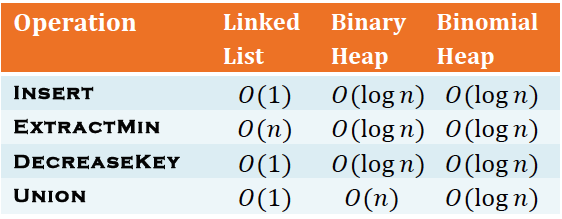
\includegraphics[width=3in]{L7-heaptablebinomialheap.png} 
	\end{center}
\end{figure}
但是对于时间复杂度的分析不是特别准确,实际上,插入操作只用了$O(1)$的时间(常数级的操作,几次就可以做到),这就是设计这个二项堆的目的,合并也是O(1)的时间。这种复杂度可以通过均摊分析来得到。
\begin{figure}[!htbp]
	\begin{center}
     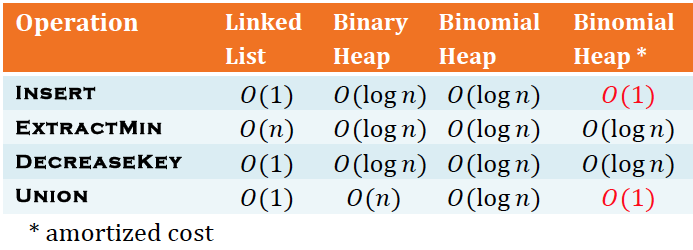
\includegraphics[width=3.4in]{L7-heaptablebinomialheap2.png} 
	\end{center}
\end{figure}

\newpage
那么什么是均摊分析?以插入操作为例,一个插入操作可能会花费非常长的时间O(log n),如图所示,插入一个值为2的节点,即$B_1$大小的树,合并形成一个$B_2$的树,继续合并最终形成一个$B_4$的树。这次插入操作挺耗时间的,但是我们注意一下,这么一次很长的插入操作之后,以后的插入操作就会
非常省事。一次插入操作之后合成一个很大的树了,那么之后再次插入就直接把$B_1$加入进去就可。所以,过去我们都是对单次操作做分析,而我们现在观察一串操作。
\begin{figure}[!htbp]
\centering
     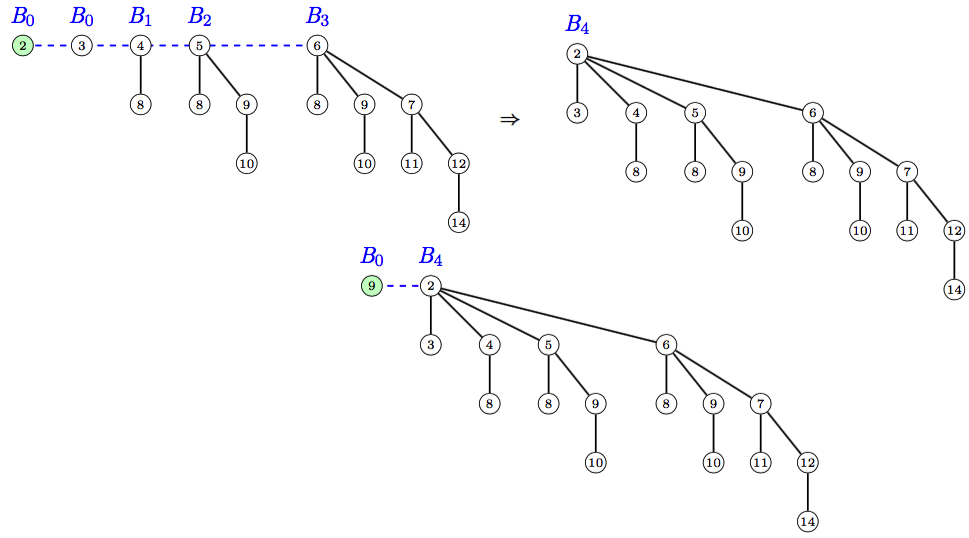
\includegraphics[width=3.9in]{L7-insertexample1.png}
\end{figure}
均摊分析的思想就是,某次操作可能花费了很长的时间,针对本例为O(log n),但是之后的操作可能就只需要O(1),O(2)。所谓均摊就是对一串操作进行平均。
下面我们用平均的思路再次看下插入操作\\
{\sc Insert}$(x)$
\begin{algorithmic}[1]
\STATE Create a $B_0$ tree for $x$;
\WHILE{ there are two $B_k$ trees for some $k$}
\STATE link them together into one $B_{k+1}$ tree; 
\ENDWHILE	
\end{algorithmic}
算法中第一句话花费O(1)的时间,While循环几次花几次时间,用w表时while循环的此时,插入操作真实的时间为1+w的时间。然后我们考虑一个量$\Phi$,称为势函数($\# tree$或树的数目)。在插入的过程当中,树的数目增加了1, whlie每循环一次减少一棵树,总减少w棵树,真实时间为1+w = 1+$\Phi$的减小值。
类似的我们看下取最小 \\
{\sc ExtractMin}$()$
\begin{algorithmic}[1]
\STATE find min of all roots; 
\STATE remove the min node; 
\WHILE{ there are two $B_k$ trees for some $k$}
\STATE link them together into one $B_{k+1}$ tree; 
\ENDWHILE	
\end{algorithmic}

把所有树的根节点拿来找最小,把最小的去掉,儿子单独成一棵树,检查将相同等级的树合并。分析时间,用w表示循环的次数,d表示取掉的最小的那个节点的儿子个数,我们同样考虑势函数$\Phi$($\#tree$或树的数目),在这个过程中,增加了d,减小了w。真实的时间为d+w=d+$\Phi$的减小值。

现在我们考虑一串的操作,包括n次插入操作和m次寻找最小的操作,总体时间花费了n*(1+decrease $\#tree$)+m*(d+decrease $\#tree$),总时间为n+m*d+所有的decrease $\#tree$,d是值删了节点会有多少节点,一个树最多有log n个儿子,所以总体时间为n+mlogn+所有减少的树。
首先注意,所有树减少的数目肯定小于增加的树的个数。那么整个树的个数增加多少?一次插入操作增加一棵,一次查最小最多增加有log n个儿子变成树,所以为n+mlogn。
所以总时间 <= 2(n+mlogn),所以平均下来,每次插入操作花费2个单位的时间,每次找最小花费2logn的时间。所以我们说均摊下来,插入操作只花费了O(1)的时间,找做小值花费了O(log n)的时间

均摊分析的定义,我们考虑一系列操作,n\_1次的操作1,n\_2次的操作2...,如果总共花费的时间为$O(n_1T_1+n_1T_2,...)$,那么我们就说操作1花费了平均T\_1的时间,操作2花费了平均T\_2的时间。
再次回顾下一次很耗时logn的插入操作之后,下面有logn级别的次数的插入操作会很小,每次几乎就是2个单位时间耗时。

\section{斐波那契堆}
但是二项堆中还有一个操作DecreaseKey(修改指定的一个值),如图把$B_4$树中的17改为1,1比16小,要调整一次,比13还小再调整一次,再继续和5调整。最后树有多高花费多少时间,即O(log n)的时间。那么DecraseKey操作能不能也快一些。确实可以,下面我们看以下斐波那契堆这种数据结构。
\begin{figure}[!htbp]
\centering
\begin{tikzpicture}[scale=1., auto,swap]

  \def\dx{0};
  \def\dy{0}; 
  \def\u{0.8};
  
   \foreach \x/\y/\name/\label in { 0/0/root/0, 0/-1/L11/8, 1/-1/L12/9, 2/-1/L13/7, 4/-1/L14/5} 
          \node[smallvertex,draw=black, fill=white!20] (\name) at (\x*\u+\dx, \y + \dy) {\tiny $\label$};
  
   \foreach \x/\y/\name/\label in {1/-2/L21/10, 2/-2/L22/11/, 3/-2/L23/12, 4/-2/L24/11, 5/-2/L25/12, 6/-2/L26/13}
          \node[smallvertex,draw=black, fill=white!20] (\name) at (\x*\u+\dx, \y + \dy) {\tiny $\label$};

   \foreach \x/\y/\name/\label in {3/-3/L31/14, 5/-3/L32/14, 6/-3/L33/15, 7/-3/L34/16}
          \node[smallvertex,draw=black, fill=white!20] (\name) at (\x*\u+\dx, \y + \dy) {\tiny $\label$};


   \foreach \x/\y/\name/\label in {7/-4/L41/17}
          \node[smallvertex,draw=black, fill=green!20] (\name) at (\x*\u+\dx, \y + \dy) {\tiny $\label$};

  
  \foreach \source/ \dest /\weight in {root/L11/{}, root/L12/{}, root/L13/{}, root/L14/{}}
         \path[undirectededge] (\source) -- node[weight] {$\weight$} (\dest);
 
  \foreach \source/ \dest /\weight in {L12/L21/{}, L13/L22/{}, L13/L23/{}, L14/L24/{}, L14/L25/{}, L14/L26/{}, L23/L31/{}, L25/L32/{}, L26/L33/{}, L26/L34/{}, L34/L41/{}}
         \path[undirectededge] (\source) -- node[weight] {$\weight$} (\dest);
 

  \node[above, blue, ultra thick] at (root.north) {$B_4$};
  
   \end{tikzpicture}
   \caption{ {\sc DecreaseKey}:   17 to 1} 
\end{figure}
那么斐波那契堆是怎么实现的呢?之前我们总是和父节点比,和父节点换,那么现在我们就不换了,单独把这个节点砍掉,称为一棵树。这种数据结构是1986年Robert Tarjan提出来的,我们看下他的基本思想,同之前一样,我们要放松下要求,一旦我们的堆序被违背之后,我们不做调整,直接砍掉。但是放松成什么样呢?过去我们的树虽然是斜着的,但是非常完美,是规整的二项式系数排列的树。现在我们不要求那么规整,但是也要和原来差不多。二项树的节点数刚好为$2^n$,现在斐波那契堆树的节点个数为$2^{1.618}$。
\subsection{斐波那契堆的Descreasekey操作}
下面看下斐波那契堆是如何操作Descreasekey的。\\
{\sc DecreaseKey}$(v, x)$
\begin{algorithmic}[1]
\STATE $key(v) = x;$
\IF{ heap order is violated}
\STATE $u = v's$ parent; 
\STATE cut subtree rooted at node $v$; 
\WHILE{ $u$ is marked} 
\STATE cut subtree rooted at node $u$, and insert it into the root list;
\STATE unmark $u$;  
\STATE $u = u's$ parent; 
\ENDWHILE	
\STATE mark $u$; 
\ENDIF
\end{algorithmic}

首先,把要求修改的那个节点v的数修改为指定的数,v的父亲节点为u,如果违反序,就把v砍掉。第五行,如果u已经被标记,干脆把u也砍掉也单独成一棵树。标记是说明该节点已经失去了一个儿子,最终的目标是每个节点最多只能丢掉一个儿子,这样树的形状不会变化的太厉害。如图是原始的斐波那契堆(从二项堆过来的):

\begin{figure}[!htbp]
\centering
\begin{tikzpicture}[scale=1., auto,swap]

  \def\dx{0};
  \def\dy{0}; 
  \def\u{0.8};
  
   \foreach \x/\y/\name/\label in { 0/0/root/0, 0/-1/L11/8, 1/-1/L12/9, 2/-1/L13/7, 4/-1/L14/5} 
          \node[smallvertex,draw=black, fill=white!20] (\name) at (\x*\u+\dx, \y + \dy) {\tiny $\label$};
  
   \foreach \x/\y/\name/\label in {1/-2/L21/10, 2/-2/L22/11/, 3/-2/L23/12, 4/-2/L24/18, 5/-2/L25/19, 6/-2/L26/13}
          \node[smallvertex,draw=black, fill=white!20] (\name) at (\x*\u+\dx, \y + \dy) {\tiny $\label$};

   \foreach \x/\y/\name/\label in {3/-3/L31/14, 5/-3/L32/20, 6/-3/L33/15, 7/-3/L34/16}
          \node[smallvertex,draw=black, fill=white!20] (\name) at (\x*\u+\dx, \y + \dy) {\tiny $\label$};


   \foreach \x/\y/\name/\label in {7/-4/L41/17}
          \node[smallvertex,draw=black, fill=white!20] (\name) at (\x*\u+\dx, \y + \dy) {\tiny $\label$};

  
  \foreach \source/ \dest /\weight in {root/L11/{}, root/L12/{}, root/L13/{}, root/L14/{}}
         \path[undirectededge] (\source) -- node[weight] {$\weight$} (\dest);
 
  \foreach \source/ \dest /\weight in {L12/L21/{}, L13/L22/{}, L13/L23/{}, L14/L24/{}, L14/L25/{}, L14/L26/{}, L23/L31/{}, L25/L32/{}, L26/L33/{}, L26/L34/{}, L34/L41/{}}
         \path[undirectededge] (\source) -- node[weight] {$\weight$} (\dest);

   \end{tikzpicture}
   \caption[1]{The original Fibonacci heap}
\end{figure}
现在想把19变成3,比父节点小砍掉,那么5失掉了一个儿子,标记为黄色。\\
\begin{figure}[!htbp]
\centering
\begin{tikzpicture}[scale=1., auto,swap]

  \def\dx{0};
  \def\dy{0}; 
  \def\u{0.8};
  
   \foreach \x/\y/\name/\label in { 0/0/root/0, 0/-1/L11/8, 1/-1/L12/9, 2/-1/L13/7, 4/-1/L14/5} 
          \node[smallvertex,draw=black, fill=white!20] (\name) at (\x*\u+\dx, \y + \dy) {\tiny $\label$};
  
   \foreach \x/\y/\name/\label in {1/-2/L21/10, 2/-2/L22/11/, 3/-2/L23/12, 4/-2/L24/18, 5/0/L3/3, 6/-2/L26/13}
          \node[smallvertex,draw=black, fill=white!20] (\name) at (\x*\u+\dx, \y + \dy) {\tiny $\label$};

   \foreach \x/\y/\name/\label in {3/-3/L31/14, 5/-1/L20/20, 6/-3/L33/15, 7/-3/L34/16}
          \node[smallvertex,draw=black, fill=white!20] (\name) at (\x*\u+\dx, \y + \dy) {\tiny $\label$};


   \foreach \x/\y/\name/\label in {7/-4/L41/17}
          \node[smallvertex,draw=black, fill=white!20] (\name) at (\x*\u+\dx, \y + \dy) {\tiny $\label$};

  
  \foreach \source/ \dest /\weight in {root/L11/{}, root/L12/{}, root/L13/{}, root/L14/{}}
         \path[undirectededge] (\source) -- node[weight] {$\weight$} (\dest);
 
  \foreach \source/ \dest /\weight in {L12/L21/{}, L13/L22/{}, L13/L23/{}, L14/L24/{}, L14/L26/{}, L23/L31/{}, L3/L20/{}, L26/L33/{}, L26/L34/{}, L34/L41/{}}
         \path[undirectededge] (\source) -- node[weight] {$\weight$} (\dest);
 


%marks
  \foreach \x/\y/\name/\label in { 4/-1/L14/5} 
          \node[smallvertex,draw=black, fill=yellow] (\name) at (\x*\u+\dx, \y + \dy) {\tiny $\label$};


  \foreach \source/ \dest /\weight in {root/L3/{}}
           \path[undirectededge, dashed, blue, thick] (\source) -- node[weight] {$\weight$} (\dest);

  
   \end{tikzpicture}
   \caption{ {\sc DecreaseKey}: 19 to 3 }
\end{figure}

现在在把15变成2,2比13小砍掉,13做上标记。
\begin{figure}[!htbp]
\centering
\begin{tikzpicture}[scale=1., auto,swap]

  \def\dx{0};
  \def\dy{0}; 
  \def\u{0.8};
  
   \foreach \x/\y/\name/\label in { 0/0/root/0, 0/-1/L11/8, 1/-1/L12/9, 2/-1/L13/7, 4/-1/L14/5} 
          \node[smallvertex,draw=black, fill=white!20] (\name) at (\x*\u+\dx, \y + \dy) {\tiny $\label$};
  
   \foreach \x/\y/\name/\label in {1/-2/L21/10, 2/-2/L22/11/, 3/-2/L23/12, 4/-2/L24/18, 5/0/L3/3, 6/-2/L26/13}
          \node[smallvertex,draw=black, fill=white!20] (\name) at (\x*\u+\dx, \y + \dy) {\tiny $\label$};

   \foreach \x/\y/\name/\label in {3/-3/L31/14, 5/-1/L20/20, 6/0/L2/2, 7/-3/L34/16}
          \node[smallvertex,draw=black, fill=white!20] (\name) at (\x*\u+\dx, \y + \dy) {\tiny $\label$};


   \foreach \x/\y/\name/\label in {7/-4/L41/17}
          \node[smallvertex,draw=black, fill=white!20] (\name) at (\x*\u+\dx, \y + \dy) {\tiny $\label$};

  
  \foreach \source/ \dest /\weight in {root/L11/{}, root/L12/{}, root/L13/{}, root/L14/{}}
         \path[undirectededge] (\source) -- node[weight] {$\weight$} (\dest);
 
  \foreach \source/ \dest /\weight in {L12/L21/{}, L13/L22/{}, L13/L23/{}, L14/L24/{}, L14/L26/{}, L23/L31/{}, L3/L20/{}, L26/L34/{}, L34/L41/{}}
         \path[undirectededge] (\source) -- node[weight] {$\weight$} (\dest);
 


%marks
  \foreach \x/\y/\name/\label in { 4/-1/L14/5, 6/-2/L13/13 } 
          \node[smallvertex,draw=black, fill=yellow] (\name) at (\x*\u+\dx, \y + \dy) {\tiny $\label$};


  \foreach \source/ \dest /\weight in {root/L3/{}, L3/L2/{}}
           \path[undirectededge, dashed, blue, thick] (\source) -- node[weight] {$\weight$} (\dest);

  
   \end{tikzpicture}
     \caption{ {\sc DecreaseKey}: 15 to 2 }

\end{figure}

再把12变为8,满足规则不做操作。

\begin{figure}[!htbp]
\centering
\begin{tikzpicture}[scale=1., auto,swap]

  \def\dx{0};
  \def\dy{0}; 
  \def\u{0.8};
  
   \foreach \x/\y/\name/\label in { 0/0/root/0, 0/-1/L11/8, 1/-1/L12/9, 2/-1/L13/7, 4/-1/L14/5} 
          \node[smallvertex,draw=black, fill=white!20] (\name) at (\x*\u+\dx, \y + \dy) {\tiny $\label$};
  
   \foreach \x/\y/\name/\label in {1/-2/L21/10, 2/-2/L22/11/, 3/-2/L23/8, 4/-2/L24/18, 5/0/L3/3, 6/-2/L26/13}
          \node[smallvertex,draw=black, fill=white!20] (\name) at (\x*\u+\dx, \y + \dy) {\tiny $\label$};

   \foreach \x/\y/\name/\label in {3/-3/L31/14, 5/-1/L20/20, 6/0/L2/2, 7/-3/L34/16}
          \node[smallvertex,draw=black, fill=white!20] (\name) at (\x*\u+\dx, \y + \dy) {\tiny $\label$};


   \foreach \x/\y/\name/\label in {7/-4/L41/17}
          \node[smallvertex,draw=black, fill=white!20] (\name) at (\x*\u+\dx, \y + \dy) {\tiny $\label$};

  
  \foreach \source/ \dest /\weight in {root/L11/{}, root/L12/{}, root/L13/{}, root/L14/{}}
         \path[undirectededge] (\source) -- node[weight] {$\weight$} (\dest);
 
  \foreach \source/ \dest /\weight in {L12/L21/{}, L13/L22/{}, L13/L23/{}, L14/L24/{}, L14/L26/{}, L23/L31/{}, L3/L20/{}, L26/L34/{}, L34/L41/{}}
         \path[undirectededge] (\source) -- node[weight] {$\weight$} (\dest);
 


%marks
  \foreach \x/\y/\name/\label in { 4/-1/L14/5, 6/-2/L13/13 } 
          \node[smallvertex,draw=black, fill=yellow] (\name) at (\x*\u+\dx, \y + \dy) {\tiny $\label$};


  \foreach \source/ \dest /\weight in {root/L3/{}, L3/L2/{}}
           \path[undirectededge, dashed, blue, thick] (\source) -- node[weight] {$\weight$} (\dest);

  
   \end{tikzpicture}
     \caption{ {\sc DecreaseKey}: 12 to 8 }

\end{figure}

再把14变为1,比8小砍掉,8做上标记。
\begin{figure}[!htbp]
\centering
\begin{tikzpicture}[scale=1., auto,swap]

  \def\dx{0};
  \def\dy{0}; 
  \def\u{0.8};
  
   \foreach \x/\y/\name/\label in { 0/0/root/0, 0/-1/L11/8, 1/-1/L12/9, 2/-1/L13/7, 4/-1/L14/5} 
          \node[smallvertex,draw=black, fill=white!20] (\name) at (\x*\u+\dx, \y + \dy) {\tiny $\label$};
  
   \foreach \x/\y/\name/\label in {1/-2/L21/10, 2/-2/L22/11/, 3/-2/L23/8, 4/-2/L24/18, 5/0/L3/3, 6/-2/L26/13}
          \node[smallvertex,draw=black, fill=white!20] (\name) at (\x*\u+\dx, \y + \dy) {\tiny $\label$};

   \foreach \x/\y/\name/\label in {-1/0/L1/1, 5/-1/L20/20, 6/0/L2/2, 7/-3/L34/16}
          \node[smallvertex,draw=black, fill=white!20] (\name) at (\x*\u+\dx, \y + \dy) {\tiny $\label$};


   \foreach \x/\y/\name/\label in {7/-4/L41/17}
          \node[smallvertex,draw=black, fill=white!20] (\name) at (\x*\u+\dx, \y + \dy) {\tiny $\label$};

  
  \foreach \source/ \dest /\weight in {root/L11/{}, root/L12/{}, root/L13/{}, root/L14/{}}
         \path[undirectededge] (\source) -- node[weight] {$\weight$} (\dest);
 
  \foreach \source/ \dest /\weight in {L12/L21/{}, L13/L22/{}, L13/L23/{}, L14/L24/{}, L14/L26/{}, L3/L20/{}, L26/L34/{}, L34/L41/{}}
         \path[undirectededge] (\source) -- node[weight] {$\weight$} (\dest);
 


%marks
  \foreach \x/\y/\name/\label in { 3/-2/L23/8, 4/-1/L14/5, 6/-2/L13/13 } 
          \node[smallvertex,draw=black, fill=yellow] (\name) at (\x*\u+\dx, \y + \dy) {\tiny $\label$};


  \foreach \source/ \dest /\weight in {L1/root/{}, root/L3/{}, L3/L2/{}}
           \path[undirectededge, dashed, blue, thick] (\source) -- node[weight] {$\weight$} (\dest);

  
   \end{tikzpicture}
     \caption{ {\sc DecreaseKey}: 14 to 1 }

\end{figure}

但是当把16变成9的时候,比13小要砍掉,但是13已经被标记了,所以把13也砍掉,5也被标记过,所以5也要被砍掉,所以最终结果为:

\begin{figure}[!htbp]
\centering
\begin{tikzpicture}[scale=1., auto,swap]

  \def\dx{0};
  \def\dy{0}; 
  \def\u{0.8};
  
   \foreach \x/\y/\name/\label in { 0/0/root/0, 0/-1/L11/8, 1/-1/L12/9, 2/-1/L7/7, 4/0/L5/5} 
          \node[smallvertex,draw=black, fill=white!20] (\name) at (\x*\u+\dx, \y + \dy) {\tiny $\label$};
  
   \foreach \x/\y/\name/\label in {1/-2/L21/10, 2/-2/L22/11/, 3/-2/L23/8, 4/-1/L24/18, 5/0/L3/3, 7/0/L13/13}
          \node[smallvertex,draw=black, fill=white!20] (\name) at (\x*\u+\dx, \y + \dy) {\tiny $\label$};

   \foreach \x/\y/\name/\label in {-1/0/L1/1, 5/-1/L20/20, 6/0/L2/2, 8/0/L9/9}
          \node[smallvertex,draw=black, fill=white!20] (\name) at (\x*\u+\dx, \y + \dy) {\tiny $\label$};


   \foreach \x/\y/\name/\label in {8/-1/L41/17}
          \node[smallvertex,draw=black, fill=white!20] (\name) at (\x*\u+\dx, \y + \dy) {\tiny $\label$};

  
  \foreach \source/ \dest /\weight in {root/L11/{}, root/L12/{}, root/L7/{}}
         \path[undirectededge] (\source) -- node[weight] {$\weight$} (\dest);
 
  \foreach \source/ \dest /\weight in {L12/L21/{}, L7/L22/{}, L7/L23/{}, L14/L24/{},  L3/L20/{}, L9/L41/{}, L5/L24/{}}
         \path[undirectededge] (\source) -- node[weight] {$\weight$} (\dest);
 


%marks
   \foreach \x/\y/\name/\label in {3/-2/L23/8}
          \node[smallvertex,draw=black, fill=yellow] (\name) at (\x*\u+\dx, \y + \dy) {\tiny $\label$};



  \foreach \source/ \dest /\weight in {L1/root/{}, root/L5/{}, L5/L3/{},  L3/L2/{}, L2/L13/{}, L13/L9/{}}
           \path[undirectededge, dashed, blue, thick] (\source) -- node[weight] {$\weight$} (\dest);

  
   \end{tikzpicture}
     \caption{ {\sc DecreaseKey}: 16 to 9 }

\end{figure}

\newpage
\subsection{斐波那契堆的插入操作}
斐波那契堆对插入操作也做了修改。如图:
\begin{figure}[!htbp]
\centering
\begin{tikzpicture}[scale=1., auto,swap]

  \def\dx{0};
  \def\dy{0}; 
  \def\u{0.8};
  
   \foreach \x/\y/\name/\label in { 0/0/root/0, 0/-1/L11/8, 1/-1/L12/9, 2/-1/L7/7, 4/0/L5/5} 
          \node[smallvertex,draw=black, fill=white!20] (\name) at (\x*\u+\dx, \y + \dy) {\tiny $\label$};
  
   \foreach \x/\y/\name/\label in {1/-2/L21/10, 2/-2/L22/11/, 3/-2/L23/8, 4/-1/L24/18, 5/0/L3/3, 7/0/L13/13}
          \node[smallvertex,draw=black, fill=white!20] (\name) at (\x*\u+\dx, \y + \dy) {\tiny $\label$};

   \foreach \x/\y/\name/\label in {-1/0/L1/1, 5/-1/L20/20, 6/0/L2/2, 8/0/L9/9}
          \node[smallvertex,draw=black, fill=white!20] (\name) at (\x*\u+\dx, \y + \dy) {\tiny $\label$};


   \foreach \x/\y/\name/\label in {8/-1/L41/17}
          \node[smallvertex,draw=black, fill=white!20] (\name) at (\x*\u+\dx, \y + \dy) {\tiny $\label$};

  
  \foreach \source/ \dest /\weight in {root/L11/{}, root/L12/{}, root/L7/{}}
         \path[undirectededge] (\source) -- node[weight] {$\weight$} (\dest);
 
  \foreach \source/ \dest /\weight in {L12/L21/{}, L7/L22/{}, L7/L23/{}, L14/L24/{},  L3/L20/{}, L9/L41/{}, L5/L24/{}}
         \path[undirectededge] (\source) -- node[weight] {$\weight$} (\dest);
 


%marks
   \foreach \x/\y/\name/\label in {3/-2/L23/8}
          \node[smallvertex,draw=black, fill=yellow] (\name) at (\x*\u+\dx, \y + \dy) {\tiny $\label$};



  \foreach \source/ \dest /\weight in {L1/root/{}, root/L5/{}, L5/L3/{},  L3/L2/{}, L2/L13/{}, L13/L9/{}}
           \path[undirectededge, dashed, blue, thick] (\source) -- node[weight] {$\weight$} (\dest);

  
   \end{tikzpicture}
\end{figure}


\begin{figure}[!htbp]
\centering
\begin{tikzpicture}[scale=1., auto,swap]

  \def\dx{0};
  \def\dy{0}; 
  \def\u{0.8};
  
   \foreach \x/\y/\name/\label in { 0/0/root/0, 0/-1/L11/8, 1/-1/L12/9, 2/-1/L7/7, 4/0/L5/5} 
          \node[smallvertex,draw=black, fill=white!20] (\name) at (\x*\u+\dx, \y + \dy) {\tiny $\label$};
  
   \foreach \x/\y/\name/\label in {1/-2/L21/10, 2/-2/L22/11/, 3/-2/L23/8, 4/-1/L24/18, 5/0/L3/3, 7/0/L13/13}
          \node[smallvertex,draw=black, fill=white!20] (\name) at (\x*\u+\dx, \y + \dy) {\tiny $\label$};

   \foreach \x/\y/\name/\label in {-1/0/L1/1, 5/-1/L20/20, 6/0/L2/2, 8/0/L9/9, 9/0/L6/6}
          \node[smallvertex,draw=black, fill=white!20] (\name) at (\x*\u+\dx, \y + \dy) {\tiny $\label$};


   \foreach \x/\y/\name/\label in {8/-1/L41/17}
          \node[smallvertex,draw=black, fill=white!20] (\name) at (\x*\u+\dx, \y + \dy) {\tiny $\label$};

  
  \foreach \source/ \dest /\weight in {root/L11/{}, root/L12/{}, root/L7/{}}
         \path[undirectededge] (\source) -- node[weight] {$\weight$} (\dest);
 
  \foreach \source/ \dest /\weight in {L12/L21/{}, L7/L22/{}, L7/L23/{}, L14/L24/{},  L3/L20/{}, L9/L41/{}, L5/L24/{}}
         \path[undirectededge] (\source) -- node[weight] {$\weight$} (\dest);
 


%marks
   \foreach \x/\y/\name/\label in {3/-2/L23/8}
          \node[smallvertex,draw=black, fill=yellow] (\name) at (\x*\u+\dx, \y + \dy) {\tiny $\label$};



  \foreach \source/ \dest /\weight in {L1/root/{}, root/L5/{}, L5/L3/{},  L3/L2/{}, L2/L13/{}, L13/L9/{}, L9/L6/{}}
           \path[undirectededge, dashed, blue, thick] (\source) -- node[weight] {$\weight$} (\dest);

  
   \end{tikzpicture}
   \caption{ {\sc Insert(6)}: creating a new tree, and insert it into the root list}
\end{figure}

比如新插入一个元素6,直接放进去就行,不像之前还需要把同级的合并,把所有的归并操作放到ExtractMin中去。这个技巧称为"Being Lazy!",
举个例子,大家书架放书,上课之前取了一本书,回来之后插入进去,但是有些同学要把书按照字母序,但是这样很累。Being Lazy 就是插入就插入,不用管它,过一周之后就自动恢复漂亮的序了。
\subsection{ExtractMin取所有节点最小}
{\sc ExtractMin}$()$
\begin{algorithmic}[1]
\STATE find min of all root nodes; 
\STATE remove the min node; 
\WHILE{ there are two roots $u$ and $v$ of the same degree} 
\STATE consolidate the two trees together;
\ENDWHILE	
\end{algorithmic}

和二项树结构找最小的操作是一样的。

\subsection{对斐波那契堆做均摊分析:这里的分析有些问题}

分析看每个操作单独花费的时间\\
观察DecraseKey单次操作实际到底花费多长时间,观察3.1中DecraseKey算法,前4行花费为O(1)时间,Whlie循环中也是单位时间,真实时间为1+w,w为whlie循环的数目。 \\
我们考察下面这个量$\Phi = \#trees+2\#marks$,表示有几棵树以及几个节点丢失了儿子。在这个过程当中,每循环一次新增了1棵树,共w棵,新增了一个标记,所以$\Phi$增量为:w+2(暂时认为为3)。
暂且认为总运行时间为:1+w=1+$\Phi$减量,但是如果我们可以把w均摊到其他操作上,那么DecraseKey操作只需要花费O(1)的时间。\\

再看下ExtractMin花费多少时间,观察3.3中的算法,第一行花费O(logn)时间,第二行花费O(logn)时间,While循环花费w时间。真实运行时间为d+w,其中d表示有多少儿子升级,放到根里面。
我们仍考察$\Phi = \#trees+2\#marks$,每次增加d棵树,每次whlie循环就减少一棵,共w棵。运行时间:d+w=d+decrease in $\Phi$。\\

再考虑插入操作,Insert操作只需要花费O(1)的时间,$\Phi$增量为1,因为增加的树的数目为1,标记没变所以$\Phi$减少量为0。

假如考虑一个操作序列包括n次插入,m次找最小,r次修改操作。整体真实运行时间为:$n+md_{max}+r+$整体$\Phi$的减少量,我们再变一下,总时间中$\Phi$减小量肯定小于增加的量,因为$\Phi$最开始为0。所以,
总运行时间小于$n+md_{max}+r+$整体$\Phi$增量。那么$\Phi$总共增加的量n*1(每次插入操作增加为1)+md\_{max}(每次找最小操作中增加为d)+3r(每次修改操作中为3,这个值有些问题)。
所以整体运行时间为:$n+md_{max}+r+n+md_{max}+3r = 2n+2md_{max}+4r$,所以平均下来,每次插入操作为O(1)单位时间,找最小值操作花费O(d\_{max}),修改操作花费O(1)的时间。

那么最后一个问题,$d_{max}$到底是多少?

对于二项树很规整,n个节点最多有$log_2n$个儿子。\\
\begin{figure}[!htbp]
\centering\
\begin{tikzpicture}[scale=0.7, auto,swap]

  \def\dx{0};
  \def\dy{0}; 
 \def\u{0.8};
  
   \foreach \x/\y/\name/\label in { 0/0/root/6, 0/-1/L11/8, 1/-1/L12/9, 2/-1/L13/7} 
          \node[smallvertex,draw=black, fill=white!20] (\name) at (\x*\u+\dx, \y + \dy) {\tiny $\label$};
  
   \foreach \x/\y/\name/\label in {1/-2/L21/10, 2/-2/L22/11/, 3/-2/L23/12}
          \node[smallvertex,draw=black, fill=white!20] (\name) at (\x*\u+\dx, \y + \dy) {\tiny $\label$};

   \foreach \x/\y/\name/\label in {3/-3/L31/14}
          \node[smallvertex,draw=black, fill=white!20] (\name) at (\x*\u+\dx, \y + \dy) {\tiny $\label$};

  
  \foreach \source/ \dest /\weight in {root/L11/{}, root/L12/{}, root/L13/{}}
         \path[undirectededge] (\source) -- node[weight] {$\weight$} (\dest);
 
  \foreach \source/ \dest /\weight in {L12/L21/{}, L13/L22/{}, L13/L23/{}, L23/L31/{}}
         \path[undirectededge] (\source) -- node[weight] {$\weight$} (\dest);
 

  %\node[above, blue, ultra thick] at (root.north) {$B_3$};
  
   \end{tikzpicture}
\end{figure}

而对于斐波那契堆,9有可能损失儿子,7有可能丢了一个儿子,最终这个树被砍成如图所示: \\
\begin{figure}[!htbp]
\centering
\begin{tikzpicture}[scale=0.7, auto,swap]

  \def\dx{0};
  \def\dy{0}; 
 \def\u{0.8};
  
   \foreach \x/\y/\name/\label in { 0/0/root/6, 0/-1/L11/8, 1/-1/L12/9, 2/-1/L13/7} 
          \node[smallvertex,draw=black, fill=white!20] (\name) at (\x*\u+\dx, \y + \dy) {\tiny $\label$};

   \foreach \x/\y/\name/\label in { 1/-1/L12/9, 2/-1/L13/7} 
          \node[smallvertex,draw=black, fill=yellow] (\name) at (\x*\u+\dx, \y + \dy) {\tiny $\label$};
  
%   \foreach \x/\y/\name/\label in {1/-2/L21/10, 2/-2/L22/11/, 3/-2/L23/12}
   \foreach \x/\y/\name/\label in { 2/-2/L22/11/}
          \node[smallvertex,draw=black, fill=white!20] (\name) at (\x*\u+\dx, \y + \dy) {\tiny $\label$};
%
%   \foreach \x/\y/\name/\label in {3/-3/L31/14}
%          \node[smallvertex,draw=black, fill=white!20] (\name) at (\x*\u+\dx, \y + \dy) {\tiny $\label$};

  
  \foreach \source/ \dest /\weight in {root/L11/{}, root/L12/{}, root/L13/{}}
         \path[undirectededge] (\source) -- node[weight] {$\weight$} (\dest);

%  \foreach \source/ \dest /\weight in {L12/L21/{}, L13/L22/{}, L13/L23/{}, L23/L31/{}}
  \foreach \source/ \dest /\weight in { L13/L22/{}}
         \path[undirectededge] (\source) -- node[weight] {$\weight$} (\dest);
 

 % \node[above, blue, ultra thick] at (root.north) {$T_3$};
  
   \end{tikzpicture}
\end{figure}

我们砍的没太狠,每个节点最多丢失一个儿子,所以d比二项树大一点,$log_{\Phi}n \geqslant d \geqslant log_2n$,其中$\Phi=\frac{1+\sqrt{5}}{2}=1.618$ \\
下面严格证明下斐波那契堆这种结构的性质。
在二项树的第i个儿子有几个孙子,第第一个儿子有0个孙子,第1个儿子有1个孙子,第二个儿子有2个孙子,所以第i个儿子有准确的i-1个孙子。如图:

\begin{figure}[!htbp]
\centering
\begin{tikzpicture}[scale=0.7, auto,swap]

  \def\dx{0};
  \def\dy{0}; 
 \def\u{0.8};
  
   \foreach \x/\y/\name/\label in { 0/0/root/6, 0/-1/L11/8, 1/-1/L12/9, 2/-1/L13/7} 
          \node[smallvertex,draw=black, fill=white!20] (\name) at (\x*\u+\dx, \y + \dy) {\tiny $\label$};
  
   \foreach \x/\y/\name/\label in {1/-2/L21/10, 2/-2/L22/11/, 3/-2/L23/12}
          \node[smallvertex,draw=black, fill=white!20] (\name) at (\x*\u+\dx, \y + \dy) {\tiny $\label$};

   \foreach \x/\y/\name/\label in {3/-3/L31/14}
          \node[smallvertex,draw=black, fill=white!20] (\name) at (\x*\u+\dx, \y + \dy) {\tiny $\label$};

  
  \foreach \source/ \dest /\weight in {root/L11/{}, root/L12/{}, root/L13/{}}
         \path[undirectededge] (\source) -- node[weight] {$\weight$} (\dest);
 
  \foreach \source/ \dest /\weight in {L12/L21/{}, L13/L22/{}, L13/L23/{}, L23/L31/{}}
         \path[undirectededge] (\source) -- node[weight] {$\weight$} (\dest);
 

  %\node[above, blue, ultra thick] at (root.north) {$B_3$};

   \end{tikzpicture}
\end{figure}
而在斐波那契堆树中,没有这么好的性质,第i个儿子至少有i-2个孙子,如图 \\
\begin{figure}[!htbp]
\centering
\begin{tikzpicture}[scale=0.7, auto,swap]

  \def\dx{0};
  \def\dy{0}; 
 \def\u{0.8};
  
   \foreach \x/\y/\name/\label in { 0/0/root/6, 0/-1/L11/8, 1/-1/L12/9, 2/-1/L13/7} 
          \node[smallvertex,draw=black, fill=white!20] (\name) at (\x*\u+\dx, \y + \dy) {\tiny $\label$};

   \foreach \x/\y/\name/\label in { 1/-1/L12/9, 2/-1/L13/7} 
          \node[smallvertex,draw=black, fill=yellow] (\name) at (\x*\u+\dx, \y + \dy) {\tiny $\label$};
  
%   \foreach \x/\y/\name/\label in {1/-2/L21/10, 2/-2/L22/11/, 3/-2/L23/12}
   \foreach \x/\y/\name/\label in { 2/-2/L22/11/}
          \node[smallvertex,draw=black, fill=white!20] (\name) at (\x*\u+\dx, \y + \dy) {\tiny $\label$};
%
%   \foreach \x/\y/\name/\label in {3/-3/L31/14}
%          \node[smallvertex,draw=black, fill=white!20] (\name) at (\x*\u+\dx, \y + \dy) {\tiny $\label$};

  
  \foreach \source/ \dest /\weight in {root/L11/{}, root/L12/{}, root/L13/{}}
         \path[undirectededge] (\source) -- node[weight] {$\weight$} (\dest);

%  \foreach \source/ \dest /\weight in {L12/L21/{}, L13/L22/{}, L13/L23/{}, L23/L31/{}}
  \foreach \source/ \dest /\weight in { L13/L22/{}}
         \path[undirectededge] (\source) -- node[weight] {$\weight$} (\dest);
 

 % \node[above, blue, ultra thick] at (root.north) {$T_3$};
   \end{tikzpicture}
\end{figure}

为什么会这样?我们考察u时w的第i个儿子,如果w当前不是一个根节点而且它最多丢失一个儿子。u是什么时候称为w的儿子呢,在合并的时候。w一开始应当有8,9这些儿子,新来的u这棵树合并起来。
我们考虑把u合并到w上那个时刻,w至少有i-1个儿子(u是第i个,此时u还没合并进来)。u当时肯定有两个儿子,不过后来丢掉了一个。因为相同级别的才会合并,所以合并的时刻degree(u)=degree(w)$\geqslant i-1$,而后面的u最多失去一个儿子,所以degree(u)$\geqslant i-2$ \\

\begin{figure}[!htbp]
\centering
\begin{tikzpicture}[scale=0.7, auto,swap]

  \def\dx{0};
  \def\dy{0}; 
 \def\u{0.8};
  
   \foreach \x/\y/\name/\label in { 0/0/root/6, 0/-1/L11/8, 1/-1/L12/9, 2/-1/L13/7} 
          \node[smallvertex,draw=black, fill=white!20] (\name) at (\x*\u+\dx, \y + \dy) {\tiny $\label$};

   \foreach \x/\y/\name/\label in { 1/-1/L12/9, 2/-1/L13/7} 
          \node[smallvertex,draw=black, fill=yellow] (\name) at (\x*\u+\dx, \y + \dy) {\tiny $\label$};
  
%   \foreach \x/\y/\name/\label in {1/-2/L21/10, 2/-2/L22/11/, 3/-2/L23/12}
   \foreach \x/\y/\name/\label in { 2/-2/L22/11/}
          \node[smallvertex,draw=black, fill=white!20] (\name) at (\x*\u+\dx, \y + \dy) {\tiny $\label$};
%
%   \foreach \x/\y/\name/\label in {3/-3/L31/14}
%          \node[smallvertex,draw=black, fill=white!20] (\name) at (\x*\u+\dx, \y + \dy) {\tiny $\label$};

  
  \foreach \source/ \dest /\weight in {root/L11/{}, root/L12/{}, root/L13/{}}
         \path[undirectededge] (\source) -- node[weight] {$\weight$} (\dest);

%  \foreach \source/ \dest /\weight in {L12/L21/{}, L13/L22/{}, L13/L23/{}, L23/L31/{}}
  \foreach \source/ \dest /\weight in { L13/L22/{}}
         \path[undirectededge] (\source) -- node[weight] {$\weight$} (\dest);
 

  \node[right, blue, ultra thick] at (root.east) {$w$};
  \node[right, blue, ultra thick] at (L13.east) {$u$};
    
\end{tikzpicture}
\end{figure}
\newpage
我们考察如下图所示的树,$B_1$有两个儿子,$B_1$最多可以丢掉一个儿子,所以B变成了$F_0$ \\
\begin{figure}[!htbp]
\centering
\begin{minipage}{0.45\textwidth}%
\begin{tikzpicture}[scale=1., auto,swap]

  \def\dx{0};
  \def\dy{0}; 
 \def\u{0.8};
  
   \foreach \x/\y/\name/\label in { 0/0/root/6, 0/-1/L11/8}
          \node[smallvertex,draw=black, fill=white!20] (\name) at (\x*\u+\dx, \y + \dy) {\tiny $\label$};
  

  
  \foreach \source/ \dest /\weight in {root/L11/{}}
         \path[undirectededge] (\source) -- node[weight] {$\weight$} (\dest);
 

  \node[above, blue, ultra thick] at (root.north) {$B_1$};
  
\end{tikzpicture}

\end{minipage}
\begin{minipage}{0.45\textwidth}%
\begin{tikzpicture}[scale=1., auto,swap]

  \def\dx{0};
  \def\dy{0}; 
 \def\u{0.8};
  
   \foreach \x/\y/\name/\label in { 0/0/root/6}
          \node[smallvertex,draw=black, fill=white!20] (\name) at (\x*\u+\dx, \y + \dy) {\tiny $\label$};
  
  \node[above, blue, ultra thick] at (root.north) {$F_0$};
  
   \end{tikzpicture}
\end{minipage}
\caption{$|B_1| = 2^1$ and $ |F_0| = 1 \geq \phi^0$}
\end{figure}

再看这幅图,我们考虑$B_2$丢失儿子最大的情况,把9那个儿子丢掉,变成$F_1$
\begin{figure}[!htbp]
\centering
\begin{minipage}{0.45\textwidth}%
\begin{tikzpicture}[scale=1., auto,swap]

  \def\dx{0};
  \def\dy{0}; 
 \def\u{0.8};
  
   \foreach \x/\y/\name/\label in { 0/0/root/6, 0/-1/L11/8, 1/-1/L12/9, 1/-2/L21/10}
          \node[smallvertex,draw=black, fill=white!20] (\name) at (\x*\u+\dx, \y + \dy) {\tiny $\label$};
  

  
  \foreach \source/ \dest /\weight in {root/L11/{}, root/L12/{}}
         \path[undirectededge] (\source) -- node[weight] {$\weight$} (\dest);
 
 

  \foreach \source/ \dest /\weight in {L12/L21/{}}
         \path[undirectededge] (\source) -- node[weight] {$\weight$} (\dest);
 


  \node[above, blue, ultra thick] at (root.north) {$B_2$};
  
  
\end{tikzpicture}

\end{minipage}
\begin{minipage}{0.45\textwidth}%
\begin{tikzpicture}[scale=1., auto,swap]

  \def\dx{0};
  \def\dy{0}; 
 \def\u{0.8};
  
   \foreach \x/\y/\name/\label in { 0/0/root/6, 0/-1/L11/8}
          \node[smallvertex,draw=black, fill=white!20] (\name) at (\x*\u+\dx, \y + \dy) {\tiny $\label$};
  

  
  \foreach \source/ \dest /\weight in {root/L11/{}}
         \path[undirectededge] (\source) -- node[weight] {$\weight$} (\dest);
 

  \node[above, blue, ultra thick] at (root.north) {$F_1$};
  


   \end{tikzpicture}

\end{minipage}
\caption{$|B_2| = 2^2$ and   $|F_1| = 2  \geq \phi^1 $}
\end{figure}

再考虑$B_3$,考虑损失儿子最狠的情况,6可以把儿子7丢掉,而9也还可以丢掉儿子10,所以最终结果为$F_2$
\begin{figure}[!htbp]
\centering
\begin{minipage}{0.45\textwidth}%
\begin{tikzpicture}[scale=1., auto,swap]

  \def\dx{0};
  \def\dy{0}; 
 \def\u{0.8};
  
   \foreach \x/\y/\name/\label in { 0/0/root/6, 0/-1/L11/8, 1/-1/L12/9, 2/-1/L13/7} 
          \node[smallvertex,draw=black, fill=white!20] (\name) at (\x*\u+\dx, \y + \dy) {\tiny $\label$};
  
   \foreach \x/\y/\name/\label in {1/-2/L21/10, 2/-2/L22/11/, 3/-2/L23/12}
          \node[smallvertex,draw=black, fill=white!20] (\name) at (\x*\u+\dx, \y + \dy) {\tiny $\label$};

   \foreach \x/\y/\name/\label in {3/-3/L31/14}
          \node[smallvertex,draw=black, fill=white!20] (\name) at (\x*\u+\dx, \y + \dy) {\tiny $\label$};

  
  \foreach \source/ \dest /\weight in {root/L11/{}, root/L12/{}, root/L13/{}}
         \path[undirectededge] (\source) -- node[weight] {$\weight$} (\dest);
 
  \foreach \source/ \dest /\weight in {L12/L21/{}, L13/L22/{}, L13/L23/{}, L23/L31/{}}
         \path[undirectededge] (\source) -- node[weight] {$\weight$} (\dest);
 

  \node[above, blue, ultra thick] at (root.north) {$B_3$};
  

  
   \end{tikzpicture}
\end{minipage}
\begin{minipage}{0.45\textwidth}%
\begin{tikzpicture}[scale=1., auto,swap]

  \def\dx{0};
  \def\dy{0}; 
 \def\u{0.8};
  
   \foreach \x/\y/\name/\label in { 0/0/root/6, 0/-1/L11/8, 1/-1/L12/9}%, 1/-2/L21/10}
          \node[smallvertex,draw=black, fill=white!20] (\name) at (\x*\u+\dx, \y + \dy) {\tiny $\label$};
  
   \foreach \x/\y/\name/\label in { 1/-1/L12/9}%, 1/-2/L21/10}
          \node[smallvertex,draw=black, fill=yellow] (\name) at (\x*\u+\dx, \y + \dy) {\tiny $\label$};
  

  
  \foreach \source/ \dest /\weight in {root/L11/{}, root/L12/{}}
         \path[undirectededge] (\source) -- node[weight] {$\weight$} (\dest);
 
 
%
%  \foreach \source/ \dest /\weight in {L12/L21/{}}
%         \path[undirectededge] (\source) -- node[weight] {$\weight$} (\dest);
% 


  \node[above, blue, ultra thick] at (root.north) {$F_2$};
  
  
   \end{tikzpicture}
   \end{minipage}
   \caption{$|B_3| = 2^3$ and   $|F_2| = 3  \geq \phi^2 $}
\end{figure}

对于$B_4$来说,丢失儿子最恨的情况,首先可以丢失最大的儿子5,然后节点7还可以丢失儿子12,然后9还可以再丢掉儿子10,最终为$F_3$。对于B\_4这棵树来说非常完美,节点个数为2\^4,而F\_3有5个
节点,个数肯定大于等于$\Phi^3$
\begin{figure}[!htbp]
\centering
\begin{minipage}{0.45\textwidth}
\begin{tikzpicture}[scale=0.7, auto,swap]

  \def\dx{0};
  \def\dy{0}; 
  \def\u{0.8};
  
   \foreach \x/\y/\name/\label in { 0/0/root/0, 0/-1/L11/8, 1/-1/L12/9, 2/-1/L13/7, 4/-1/L14/5} 
          \node[smallvertex,draw=black, fill=white!20] (\name) at (\x*\u+\dx, \y + \dy) {\tiny $\label$};
  
   \foreach \x/\y/\name/\label in {1/-2/L21/10, 2/-2/L22/11/, 3/-2/L23/12, 4/-2/L24/11, 5/-2/L25/12, 6/-2/L26/13}
          \node[smallvertex,draw=black, fill=white!20] (\name) at (\x*\u+\dx, \y + \dy) {\tiny $\label$};

   \foreach \x/\y/\name/\label in {3/-3/L31/14, 5/-3/L32/14, 6/-3/L33/15, 7/-3/L34/16}
          \node[smallvertex,draw=black, fill=white!20] (\name) at (\x*\u+\dx, \y + \dy) {\tiny $\label$};


   \foreach \x/\y/\name/\label in {7/-4/L41/17}
          \node[smallvertex,draw=black, fill=white!20] (\name) at (\x*\u+\dx, \y + \dy) {\tiny $\label$};

  
  \foreach \source/ \dest /\weight in {root/L11/{}, root/L12/{}, root/L13/{}, root/L14/{}}
         \path[undirectededge] (\source) -- node[weight] {$\weight$} (\dest);
 
  \foreach \source/ \dest /\weight in {L12/L21/{}, L13/L22/{}, L13/L23/{}, L14/L24/{}, L14/L25/{}, L14/L26/{}, L23/L31/{}, L25/L32/{}, L26/L33/{}, L26/L34/{}, L34/L41/{}}
         \path[undirectededge] (\source) -- node[weight] {$\weight$} (\dest);
 

  \node[above, blue, ultra thick] at (root.north) {$B_4$};
  

  
   \end{tikzpicture}
   \end{minipage}
   \begin{minipage}{0.45\textwidth}
\begin{tikzpicture}[scale=1., auto,swap]

  \def\dx{0};
  \def\dy{0}; 
 \def\u{0.8};
  
   \foreach \x/\y/\name/\label in { 0/0/root/6, 0/-1/L11/8, 1/-1/L12/9, 2/-1/L13/7} 
          \node[smallvertex,draw=black, fill=white!20] (\name) at (\x*\u+\dx, \y + \dy) {\tiny $\label$};

   \foreach \x/\y/\name/\label in { 1/-1/L12/9, 2/-1/L13/7} 
          \node[smallvertex,draw=black, fill=yellow] (\name) at (\x*\u+\dx, \y + \dy) {\tiny $\label$};
  
%   \foreach \x/\y/\name/\label in {1/-2/L21/10, 2/-2/L22/11/, 3/-2/L23/12}
   \foreach \x/\y/\name/\label in { 2/-2/L22/11/}
          \node[smallvertex,draw=black, fill=white!20] (\name) at (\x*\u+\dx, \y + \dy) {\tiny $\label$};
%
%   \foreach \x/\y/\name/\label in {3/-3/L31/14}
%          \node[smallvertex,draw=black, fill=white!20] (\name) at (\x*\u+\dx, \y + \dy) {\tiny $\label$};

  
  \foreach \source/ \dest /\weight in {root/L11/{}, root/L12/{}, root/L13/{}}
         \path[undirectededge] (\source) -- node[weight] {$\weight$} (\dest);

%  \foreach \source/ \dest /\weight in {L12/L21/{}, L13/L22/{}, L13/L23/{}, L23/L31/{}}
  \foreach \source/ \dest /\weight in { L13/L22/{}}
         \path[undirectededge] (\source) -- node[weight] {$\weight$} (\dest);
 

  \node[above, blue, ultra thick] at (root.north) {$F_3$};
  

  
   \end{tikzpicture}   
    \end{minipage}
    \caption{$|B_4| = 2^4$ and   $|F_3| = 5  \geq \phi^3 $}
\end{figure}

再看这个递归的画法,B\_5的节点个数为2\^5,F\_4的节点个数为8,肯定小于等于$\Phi^4$。我们可以观察到,从$F_0$到$F_4$,节点个数为1,2,3,5,8,也就是说满足这种规则的最小的树的节点的数目为斐波那契数。
所以任何一棵树的规模大于等于$\Phi^k$,所以$d_max \leqq log_\Phi n$。

\begin{figure}[!htbp]
\centering
   \begin{minipage}{0.45\textwidth}

\begin{tikzpicture}[scale=0.7, auto,swap]

  \def\dx{0};
  \def\dy{0}; 
  \def\u{0.8};
  
  
   \draw[thick, fill=green!20] (6+\dx, -1+\dy) -- (6-0.5+\dx, -1-0.73+\dy) -- (6.5+\dx, -1-0.73+\dy) -- (6+\dx,-1+\dy); 
   \node[ thick, blue] at (6+\dx, -1-0.48+\dy) { $B_4$};

   \foreach \x/\y/\name/\label in { 0/0/root/0, 0/-1/L11/8, 1/-1/L12/9, 2/-1/L13/7, 4/-1/L14/5, 7.5/-1/L15/6} 
          \node[smallvertex,draw=black, fill=white!20] (\name) at (\x*\u+\dx, \y + \dy) {\tiny $\label$};
  
   \foreach \x/\y/\name/\label in {1/-2/L21/10, 2/-2/L22/11/, 3/-2/L23/12, 4/-2/L24/11, 5/-2/L25/12, 6/-2/L26/13}
          \node[smallvertex,draw=black, fill=white!20] (\name) at (\x*\u+\dx, \y + \dy) {\tiny $\label$};

   \foreach \x/\y/\name/\label in {3/-3/L31/14, 5/-3/L32/14, 6/-3/L33/15, 7/-3/L34/16}
          \node[smallvertex,draw=black, fill=white!20] (\name) at (\x*\u+\dx, \y + \dy) {\tiny $\label$};


   \foreach \x/\y/\name/\label in {7/-4/L41/17}
          \node[smallvertex,draw=black, fill=white!20] (\name) at (\x*\u+\dx, \y + \dy) {\tiny $\label$};

  
  \foreach \source/ \dest /\weight in {root/L11/{}, root/L12/{}, root/L13/{}, root/L14/{}, root/L15/{}}
         \path[undirectededge] (\source) -- node[weight] {$\weight$} (\dest);
 
  \foreach \source/ \dest /\weight in {L12/L21/{}, L13/L22/{}, L13/L23/{}, L14/L24/{}, L14/L25/{}, L14/L26/{}, L23/L31/{}, L25/L32/{}, L26/L33/{}, L26/L34/{}, L34/L41/{}}
         \path[undirectededge] (\source) -- node[weight] {$\weight$} (\dest);
 
 

  \node[above, blue, ultra thick] at (root.north) {$B_5$};
  

  
   \end{tikzpicture}
   
   \end{minipage}
   \begin{minipage}{0.45\textwidth}

\begin{tikzpicture}[scale=1., auto,swap]

  \def\dx{0};
  \def\dy{0}; 
  \def\u{0.8};
  
   \foreach \x/\y/\name/\label in { 0/0/root/0, 0/-1/L11/8, 1/-1/L12/9, 2/-1/L13/7, 4/-1/L14/5} 
          \node[smallvertex,draw=black, fill=white!20] (\name) at (\x*\u+\dx, \y + \dy) {\tiny $\label$};
  
   \foreach \x/\y/\name/\label in {2/-2/L22/11/, 4/-2/L24/11, 5/-2/L25/12}
          \node[smallvertex,draw=black, fill=white!20] (\name) at (\x*\u+\dx, \y + \dy) {\tiny $\label$};



   \foreach \x/\y/\name/\label in { 1/-1/L12/9, 2/-1/L13/7, 4/-1/L14/5,5/-2/L25/12} 
          \node[smallvertex,draw=black, fill=yellow] (\name) at (\x*\u+\dx, \y + \dy) {\tiny $\label$};
  

  
  \foreach \source/ \dest /\weight in {root/L11/{}, root/L12/{}, root/L13/{}, root/L14/{}}
         \path[undirectededge] (\source) -- node[weight] {$\weight$} (\dest);
 
  \foreach \source/ \dest /\weight in {L13/L22/{},  L14/L24/{}, L14/L25/{}}
         \path[undirectededge] (\source) -- node[weight] {$\weight$} (\dest);
 

  \node[above, blue, ultra thick] at (root.north) {$F_4$};
  

  
   \end{tikzpicture}

   \end{minipage}
   \caption{$|B_5| = 2^5$ and   $|F_4| = 8  \geq \phi^4$}

\end{figure}
所以斐波那契堆的复杂度:插入仍未为O(1),取最小仍未O(nlogn),合并为O(1),而DecreaseKey的操作变成了O(1)的时间,为什么,变化某个数之后,只要违反了堆序,根本不去调整,直接当成一棵树,所以平均下来为O(1)的时间。\\
\begin{figure}[!htbp]
\centering
	\begin{center}
     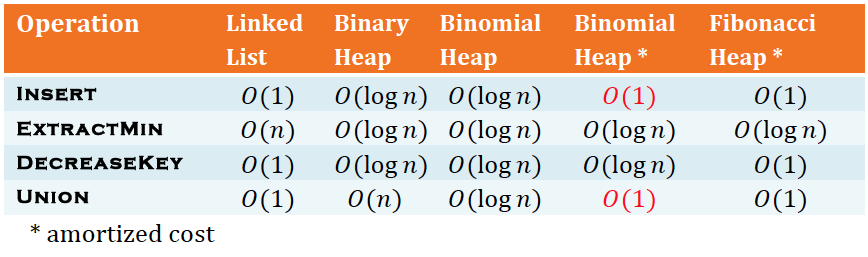
\includegraphics[width=4in]{L7-heaptablefibonacciheap.png} 
	\end{center}
\end{figure}


那么DecreaseKey的操作变为O(1)后对我们的算法有什么影响呢?Dijstra算法的运行时间从最开始数组结构的O(n\^2),到二叉堆的O(mlogn),到二项堆的O(mlogn),到最终斐波那契堆的O(m+nlogn)。
时间复杂度好了很多。

  \begin{table}
  \begin{tabular}{crrrr}
  \hline  \hline
  Operation & Linked  & Binary  & Binomial  & Fibonacci  \\
            &  list &  heap &  heap & heap \\
  \hline
  {\sc MakeHeap} & $ 1 $ &  $1$  & $ 1 $ & $1$  \\ 
  {\sc Insert} & $ 1 $ &  $\log n$  & $ \log n $ & $1$  \\ 
   {\sc ExtractMin} & $ n $ &  $\log n$  & $ \log n  $ & $ \log n $  \\ 
  {\sc DecreaseKey} & $ 1 $ &  $\log n$  & $ \log n $ & $1$  \\ 
  {\sc Delete} & $ n $ &  $\log n$  & $ \log n $ & $\log n$  \\ 
  {\sc Union} & $ 1 $ &  $ n $  & $ \log n $ & $1$  \\ 
   {\sc FindMin} & $ n $ &  $1$  & $ \log n $ & $1$  \\ 
  \hline 
  {\sc Dijkstra} & $ O(n^2) $ &  $ O(m \log n) $  & $ O( m \log n ) $ & $ O( m + n \log n) $  \\ 
  \hline \hline 
  \end{tabular} 
  \end{table}
{\sc Dijkstra} algorithm: $n$ {\sc Insert}, $n$ {\sc ExtractMin}, and $m$ {\sc DecreaseKey}. 

\section{Greedy贪心算法}
贪心算法经常是每一步都选择局部最优的,是非常短视的(Near Sight),希望每次局部的最优最终能够达到全局最优。那么一个贪心算法应该怎么做呢,什么时候用?
假如说我们观察到我们问题的解是$X=[x_1,x_2,...x_n]$,每个$x_i \in S_i$,我们的目标时要找$X^*$ 使得$X^*$ 为最大值。凡是我们碰到问题的解是由多项组成的,我们要考虑两招:一招是枚举,另一招就是贪心。
这里有一个关键概念称为“部分解树”,我们的解太大不好找,我们让解慢慢的长起来,如图,解从空开始,不断往下延伸,每个中间节点都是一个部分解,叶子节点是一个完整的解,我们最终从叶子节点中找到最优的。
每次遇到这里问题可以画类似的图。第一招枚举所有的叶子节点,但是太慢,我们第一节提到多可以剪枝来减少规模,不用枚举所有的。第二招我们在第一个节点可以选择到底时让x等于1还是0,根据当前的状态判断必然选0,那么选0后在根据状态来判断
必然要往下走,所以这是沿着一个或者多条路径来往下走。

 \begin{figure}[!htbp]
 \centering
\begin{tikzpicture}[scale=1., auto,swap]
    % Draw a 7,11 network
    % First we draw the vertices
    \foreach \pos/\name in {{(0,0)/A1234}, {(-1,-1)/A12}, {(1,-1)/A34}, {(-1.5,-2)/A1}, {(-.5, -2)/A2}, {(0.5, -2)/A3}, {(1.5, -2)/A4}}
        \node[smallvertex,draw=black, fill=blue!20] (\name) at \pos {};
    % Connect vertices with edges and draw weights
    \foreach \source/ \dest /\weight in {A1234/A12/{}, A1234/A34/{}, A12/A1/{}, A12/A2/{}, A34/A3/{}, A34/A4/{}  }
        \path[undirectededge] (\source) -- node[weight] {$\weight$} (\dest);
%       \draw[dashed, ->] (0,0) arc  (120:60:2);
 
   \node[above] at (0,0.2) {\tiny $ \Phi $};
   \node[left] at (-1.2, -1) {\tiny $ [0] $};
   \node[right] at (1.2, -1) {\tiny $ [1]$};
   \node[below] at (-1.5, -2.2) {\tiny $ [0, 0]$};
   \node[below] at (-.5, -2.2) {\tiny $[0, 1]$};
   \node[below] at (.5, -2.2) {\tiny $[1, 0]$};
   \node[below] at (1.5, -2.2) {\tiny $[1, 1]$};
   \end{tikzpicture}
\end{figure}

下面我们看一个例子,给我们上课起止的时间,每堂课容纳的学生都为w=1,让我们找选择那些课使得不冲突可以使最多的学生上课。我们遵循是$X=[x_1,x_2,...x_n]$,那么\\
$x_1 \in [1,2,..9]$,如果$x_1$选择1之后,$x_2 \in [3,4,5,7,8,9]$,以此我们可以把整个树枚举出来,最后在叶子节点中找到最大的那个。那么贪心怎么操作,对于空的时候,就觉得第一个选择1,不枚举所有的树,其他都不用扩展,贪心选择1
之后,我们选择3,3再往下扩展到最终的叶子节点。所谓贪心就是在部分解树中找了一条路径。

\begin{figure}[!htbp]
\centering
 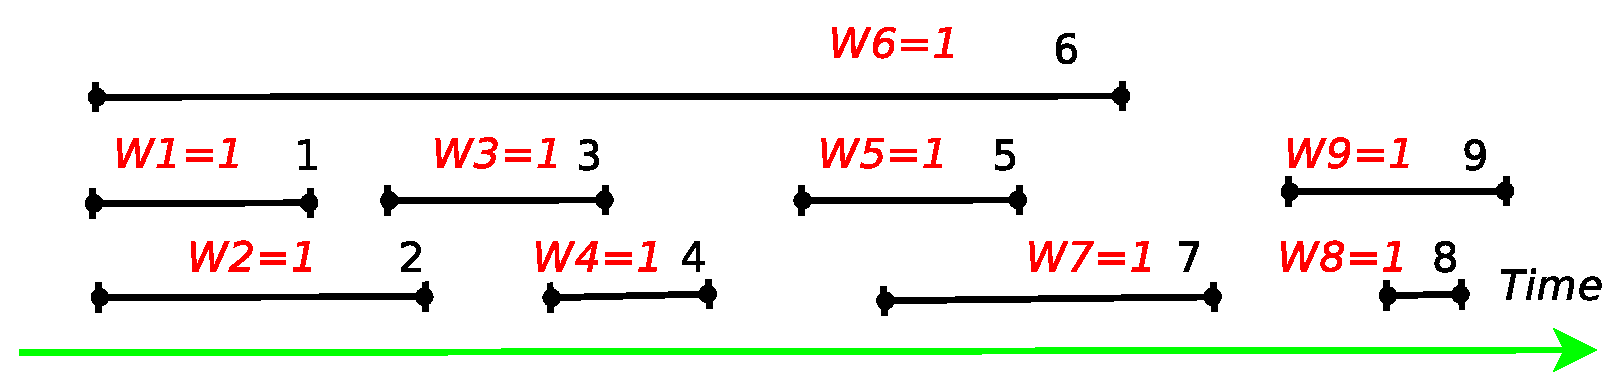
\includegraphics[width=4in] {L7-intervalschedulingexampleall1.eps}
\end{figure}

我们再来看TSP问题,如图

\begin{figure}[!htbp]
\centering
	\begin{tikzpicture}[scale=1, auto,swap]

    \foreach \pos/ \name in {{(0,0)/b},{(0,2)/a}, {(2,2)/d}, {(2,0)/c}} 
        \node[smallvertex,fill=blue!20] (\name) at \pos{$\name$};

     
    % Connect vertices with edges and draw weights
    \foreach \source/ \dest/\weight in {b/a/{1},   b/c/{4}, a/d/{5}, d/c/{6}}
        \path[undirectededge] (\source) -- node[weight] {$\weight$} (\dest);
    \foreach \source/ \dest/\weight in  {a/c/{3}, b/d/{2}}
        \path[undirectededge] (\source) -- node[weight] {$\weight$} (\dest);
        
	\end{tikzpicture}
\end{figure}

$X=[x_1,x_2,...x_n]$,还是按照部分解树,先画出完整的解树,一开始解是空的$\Phi$,部分解树如图,那么贪心规则是什么呢?我们就说从a出发到下一个节点谁最短选择谁,也就是图示沿着绿色节点的路径。
而其余的分支都不再考虑。所以贪心比较快,贪心每次选择局部最优。
 \begin{figure}[!htbp]
 \centering
\begin{tikzpicture}[scale=1., auto,swap]
    % Draw a 7,11 network
    % First we draw the vertices
    \foreach \pos/\name in {{(0,0)/A123456}, {(0,-1)/A34}, {(2,-1)/A56}, {(-2.5,-2)/A1},{(-.5, -2)/A3}, {(0.5, -2)/A4}, {(1.5,-2)/A5}, {(2.5, -2)/A6},{(-2.5,-3)/A11}, {(-.5, -3)/A33}, {(0.5, -3)/A44}, {(1.5,-3)/A55}, {(2.5, -3)/A66}}
        \node[smallvertex,draw=black, fill=blue!20] (\name) at \pos {};
        
    	\foreach \pos/\name in {{(-2,-1)/A12},{(-1.5,-2)/A2},{(-1.5,-3)/A22}}
    	        \node[smallvertex,draw=black, fill=green!20] (\name) at \pos {};
    % Connect vertices with edges and draw weights
    \foreach \source/ \dest /\weight in {A123456/A12/{}, A123456/A34/{}, A123456/A56/{},A12/A1/{}, A12/A2/{}, A34/A3/{}, A34/A4/{},A56/A5/{},A56/A6/{},A1/A11/{},A2/A22/{},A3/A33/{},A4/A44/P{},A5/A55/{},A6/A66/{}}
        \path[undirectededge] (\source) -- node[weight] {$\weight$} (\dest);
%       \draw[dashed, ->] (0,0) arc  (120:60:2);

 
   \node[above] at (0,0.2) {\tiny $ \Phi $};
   \node[left] at (-0.1,-1) {b};
   \node[left] at (-2.1,-1) {c};
   \node[right] at (2.1,-1) {d};
   \node[left] at (-2.6,-2) {b};
   \node[left] at (-1.6,-2) {d};
   \node[left] at (-0.6,-2) {c};
   \node[right] at (2.6,-2) {c};
   \node[right] at (1.6,-2) {b};
   \node[right] at (0.6,-2) {d};
   
      \node[left] at (-2.6,-3) {d};
      \node[left] at (-1.6,-3) {b};
      \node[left] at (-0.6,-3) {d};
      \node[right] at (2.6,-3) {b};
      \node[right] at (1.6,-3) {c};
      \node[right] at (0.6,-3) {c};
   \end{tikzpicture}
\end{figure}

我们主要目的不是讲各种技巧,而是观察给定的问题的结构:一类是可以规约成子问题可以分,一类不可以规约就Impove,还有一类就是枚举。
\subsection{拟阵}

问题:给定一个矩阵,求极大线性无关组。如图,给定五个向量,我们还是按照上述的部分解树来看。贪心就是每次从里面选出一条路径出来,最终到叶子节点。
\begin{table}[!htbp]
{
\begin{tabular}{lrrrrrrr}
$A_{1}=[$& 1 & 2 & 3 & 4 & 5 $]$   \\ 
$A_{2}=[$& 1 & 4 & 9 & 16 & 25 $]$   \\ 
$A_{3}=[$& 1 & 8 & 27 & 64 & 125 $]$  \\ 
$A_{4}=[$& 1 & 16 & 81 & 256 & 625 $]$  \\ 
$A_{5}=[$& 2 & 6 & 12 & 20 & 30 $]$  \\ 
\end{tabular}}{}
\end{table}

算法描述如下,初始解为空,对任意的行向量,加进去一个向量,如果是线性无关,就往解集合中加。\\
{\sc IndependentSet}$( M )$
\begin{algorithmic}[1]
\STATE $A=\{ \};$
\FORALL { row vector $v $  }
\IF { $A\cup\{v\}$ is still independent }
\STATE $A=A\cup\{v\}$;
\ENDIF
\ENDFOR
\RETURN $A$;
\end{algorithmic}
因为线性无关有两个性质:\\
(1)继承性:如果B是一个线性无关组,如果$A \subset B$,那么A也是一个线性无关组。\\
(2)扩展性:如果A和B都是线性无关组,并且|A|<|B|,那么从B当中肯定能够找到一些向量加到A当中,使得A还是线性无关向量组。

考虑另一个问题:加入每个向量都关联了一个权重w,我们在这里选出一些向量出来是线性无关的,同时权重之和是最大的。如图:
\begin{table}[!htbp]{
\begin{tabular}{lrrrrrrl}
$A_{1}=[$& 1 & 2 & 3 & 4 & 5 $]$&\textcolor{red}{$W_{1}=9$} \\ 
$A_{2}=[$& 1 & 4 & 9 & 16 & 25 $]$&\textcolor{red}{$W_{2}=7$} \\ 
$A_{3}=[$& 1 & 8 & 27 & 64 & 125 $]$&\textcolor{red}{$W_{3}=5$}\\ 
$A_{4}=[$& 1 & 16 & 81 & 256 & 625 $]$&\textcolor{red}{$W_{4}=3$}\\ 
$A_{5}=[$& 2 & 6 & 12 & 20 & 30 $]$&\textcolor{red}{$W_{5}=1$}\\ 
\end{tabular}}{}
\end{table}
我们按照贪心的想法,初始解为空,每次取权重最大的那个,本例中先选A1,然后再选A2,直到线性相关就不选。算法如下,首先解为空,我们把所有的向量的按照权重做
降序排列,然后和无权重的算法一样。算法复杂度为O(nlogn+ nC(n)),O(nlogn)是排序时间,C(n)是每次检查线性无关花费多少时间。\\
{\sc Matroid\_Greedy}$( M, W )$
\begin{algorithmic}[1]
\STATE $A=\{ \};$
\STATE \textcolor{red}{\bf Sort row vectors in the decreasing order of their weights;}
\FORALL { row vector $v $  }
\IF { $A\cup\{v\}$ is still independent }
\STATE $A=A\cup\{v\}$;
\ENDIF
\ENDFOR
\RETURN $A$;
\end{algorithmic}

上述算法是对的么?首先这个算法第一是具有最优子结构的性质,第二个是具有贪心选择性质。首先v是权重最大的向量,并且v本身就是线性无关的。假设A是最优的解,且A包含v。\\
证明:我们假设存在另外一个最优结构,但是v $\notin$ B;我们从B中开始构造一个新的$A={v}$,因为B比A大,B中肯定可以挑出一个向量添加到A中,直到A和B一样多,因为极大线性无关组的数目肯定一样多(即矩阵的秩)。最后A和B元素只有一个元素不同,
因为A选择了v,所以B肯定选了另一个v',而v的权重最大,所以A的权重肯定比B大。
那么剩下的自问题就是:和v线性相关的全部去掉,剩下的作为子问题A'。因为A'中每个向量都是和v线性无关的,所以$A=A'\cup{v}$,所以A肯定也是线性无关的。这样选择每次的v都具有最大的权重,所以最终会得到最优的解。

极大线性无关组并不仅仅存在在矩阵中,同样存在在其他问题中,我们称为“拟阵”(matroid,由Haussler在1935年提出)。他发现矩阵中的线性无关概念和图论中的森林很像。如果一个图不包含回路,就称为独立。
在图当中的无环子图(森林),连同且无圈称为树,图中B所示。如果只要求无圈称为森林,图中A所示。\\

继承性:如果一个森林,挑其中几个边,仍然是个森林(和线性无关组相似)。如图:

 \begin{figure}[!htbp]
 \centering
\begin{tikzpicture}[scale=0.7, auto,swap]

   \def\dx{0};
    \node[red, ultra thick] at (1+\dx, 1) {$G$};
    \foreach \pos/\name in {{(0+\dx,0)/s}, {(2+\dx,0)/u}, {(-1+\dx, -2)/v}, {(1+\dx,-2)/w}, {(3+\dx,-2)/t}}
        \node[middlevertex,fill=blue!20] (\name) at \pos {$\name$};
        
        
    \foreach \source/\dest/\weight in {s/u/, s/w/, s/v/,  u/w/, v/w/, u/t/ } 
            \path[undirectededge] (\source) -- node{\small $\weight$} (\dest);
		
		
    \def\dx{5.5};
    \node[red, ultra thick] at (1+\dx, 1) {$B$};
    \foreach \pos/\name in {{(0+\dx,0)/s}, {(2+\dx,0)/u}, {(-1+\dx, -2)/v}, {(1+\dx,-2)/w}, {(3+\dx,-2)/t}}
        \node[middlevertex,fill=blue!20] (\name) at \pos {$\name$};
        
        
     \foreach \source/\dest/\weight in {s/u/, s/v/,  u/w/, u/t/ } 
                 \path[undirectededge] (\source) -- node{\small $\weight$} (\dest);
		
	
    \def\dx{11};
    \node[red, ultra thick] at (1+\dx, 1) {$A$};
    \foreach \pos/\name in {{(0+\dx,0)/s}, {(2+\dx,0)/u}, {(-1+\dx, -2)/v}, {(1+\dx,-2)/w}, {(3+\dx,-2)/t}}
        \node[middlevertex,fill=blue!20] (\name) at \pos {$\name$};	
        
        
     \foreach \source/\dest/\weight in { s/v/,  u/w/, u/t/ } 
            \path[undirectededge] (\source) -- node{\small $\weight$} (\dest);
                    			
		
\end{tikzpicture} 
\end{figure}    

扩展性:如果A和B都是无环森林,并且A是个小森林,那么从B中挑出一些边放到A中使得A还是森林。如图从B中添加$E_{su}$到A中形成A'。\\
如果森林B比A的边数要多($\#Tree=|V|-|E|$,V是节点,E是边),那么B的树的数目比A要少,B中肯定有一棵树是A中两棵树连接而成的。图例中的为(u,v)是跨了两棵树,所以加入到A中肯定不会形成圈。


\begin{figure}[!htbp]
\centering
\begin{tikzpicture}[scale=0.6, auto,swap]
 
 
    \def\dx{0};
    \node[red, ultra thick] at (1+\dx, 1) {$B$};
    \foreach \pos/\name in {{(0+\dx,0)/s}, {(2+\dx,0)/u}, {(-1+\dx, -2)/v}, {(1+\dx,-2)/w}, {(3+\dx,-2)/t}}
        \node[middlevertex,fill=blue!20] (\name) at \pos {$\name$};
        
        
    \foreach \source/\dest/\weight in {s/u/, u/v/,  v/w/, u/t/ } 
            \path[undirectededge] (\source) -- node{\small $\weight$} (\dest);

    \def\dx{5.5};
    \node[red, ultra thick] at (1+\dx, 1) {$A'$};
    \foreach \pos/\name in {{(0+\dx,0)/s}, {(2+\dx,0)/u}, {(-1+\dx, -2)/v}, {(1+\dx,-2)/w}, {(3+\dx,-2)/t}}
        \node[middlevertex,fill=blue!20] (\name) at \pos {$\name$};
        
        
    \foreach \source/\dest/\weight in {s/u/, s/v/,  u/w/, u/t/ } 
            \path[undirectededge] (\source) -- node{\small $\weight$} (\dest);

    \foreach \source/\dest/\weight in {s/u/ } 
            \path[undirectededge, red] (\source) -- node{\small $\weight$} (\dest);
		
		
		
    \def\dx{11};
    \node[red, ultra thick] at (1+\dx, 1) {$A$};
    \foreach \pos/\name in {{(0+\dx,0)/s}, {(2+\dx,0)/u}, {(-1+\dx, -2)/v}, {(1+\dx,-2)/w}, {(3+\dx,-2)/t}}
        \node[middlevertex,fill=blue!20] (\name) at \pos {$\name$};
        
        
    \foreach \source/\dest/\weight in { s/v/, u/w/, u/t/ } 
            \path[undirectededge] (\source) -- node{\small $\weight$} (\dest);
		

\end{tikzpicture} 
\end{figure}    

\subsection{Kruskal算法}
那么拟帧有什么用呢?我们可以看下最小支撑树的问题:在实际电路板中,焊点之间都有距离,选择那些可以把这些焊点全部连接起来使得距离最小?
\begin{figure}[!htbp]
\centering
\begin{tikzpicture}[scale=1, auto,swap]
 
    \foreach \pos/\name in {{(0,0)/a}, {(1,1)/b}, {(1 , -1)/h}, {(2,0)/i}, {(3 ,1)/c}, {(3,-1)/g}, {(5,-1)/f},{(5,1)/d},{(6,0)/e}}
        \node[middlevertex,fill=blue!20] (\name) at \pos {$\name$};
        
    \foreach \source/\dest/\weight in {b/a/4, a/h/8, h/b/11, c/b/8, i/c/2, h/i/7, g/i/6, h/g/1, g/f/2, c/f/4, d/c/7, d/f/14, e/d/9, f/e/10 } 
            \path[undirectededge] (\source) -- node{\small $\weight$} (\dest);

    \foreach \source/\dest/\weight in {a/b/, c/i/, b/c/, c/f/, f/g/, g/h/, c/d/, d/e/  } 
            \path[selected edge] (\source) -- node{\small $\weight$} (\dest);

\end{tikzpicture}
\end{figure}  

我们看下线性无关组和森林之间的关系:线性无关组对于森林。极大线性无关组对应支撑树。加权的加大线性无关组对应最小支撑树。所以我们就可以和处理加权极大线性无关组一样来处理最小支撑树。
\begin{figure}[!htbp]
 	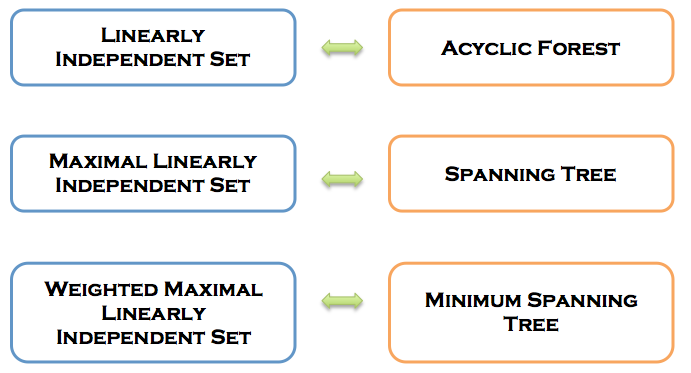
\includegraphics[width=4in]{L7-independentsetforest.png}
 \end{figure}

{\sc GenericSpanningTree}$( G )$
\begin{algorithmic}[1]
\STATE{ $F=\{ \};$ }
\WHILE{ $F$ does not form a spanning tree } 
\STATE{ find an edge $(u, v)$ that is \textcolor{red}{\bf safe} for $F$; }
\STATE{ $F = F\cup\{ (u, v) \}$; }
\ENDWHILE
\end{algorithmic}
上述算法为求支撑树,算法每次找一条边如果是safe的话就加入到F中。Safe意思就是不形成环。我们会发现和求矩阵线性无关组的算法基本一样。看下Safe和Unsafe的例子:\\
\begin{figure}[!htbp]
\centering
\begin{tikzpicture}[scale=1, auto,swap]
 
    \foreach \pos/\name in {{(0,0)/a}, {(1,1)/b}, {(1 , -1)/h}, {(2,0)/i}, {(3 ,1)/c}, {(3,-1)/g}, {(5,-1)/f},{(5,1)/d},{(6,0)/e}}
        \node[middlevertex,fill=blue!20] (\name) at \pos {$\name$};
        
    \foreach \source/\dest/\weight in {b/a/4, a/h/8, h/b/11, c/b/8, i/c/2, h/i/7, g/i/6, h/g/1, g/f/2, c/f/4, d/c/7, d/f/14, e/d/9, f/e/10 } 
            \path[undirectededge] (\source) -- node{\small $\weight$} (\dest);

    \foreach \source/\dest/\weight in {a/b/, c/i/, c/f/,  f/g/  } 
            \path[selected edge] (\source) -- node{\small $\weight$} (\dest);

    \foreach \source/\dest/\weight in {c/d/ } 
            \path[undirectededge, blue, ultra thick] (\source) -- node{\small $\weight$} (\dest);

\end{tikzpicture} 
\caption{Safe edge} 
\end{figure}   

\begin{figure}[!htbp]
\centering
\begin{tikzpicture}[scale=1, auto,swap]
 
    \foreach \pos/\name in {{(0,0)/a}, {(1,1)/b}, {(1 , -1)/h}, {(2,0)/i}, {(3 ,1)/c}, {(3,-1)/g}, {(5,-1)/f},{(5,1)/d},{(6,0)/e}}
        \node[middlevertex,fill=blue!20] (\name) at \pos {$\name$};
        
    \foreach \source/\dest/\weight in {b/a/4, a/h/8, h/b/11, c/b/8, i/c/2, h/i/7, g/i/6, h/g/1, g/f/2, c/f/4, d/c/7, d/f/14, e/d/9, f/e/10 } 
            \path[undirectededge] (\source) -- node{\small $\weight$} (\dest);

    \foreach \source/\dest/\weight in {a/b/, c/i/, c/f/, f/g/ } 
            \path[selected edge] (\source) -- node{\small $\weight$} (\dest);

    \foreach \source/\dest/\weight in {g/i/ } 
            \path[undirectededge, blue, ultra thick] (\source) -- node{\small $\weight$} (\dest);

\end{tikzpicture}
\caption{Unsafe edge}  
\end{figure}   

求支撑树我们已经会求了,那么最小支撑树呢?Kruskal在1956年提出来的算法。\\
{\sc MST-Kruskal}$( G, W )$
\begin{algorithmic}[1]
\STATE{ $F = \{ \}; $} 
\FORALL{ vertex $v \in V$ } 
\STATE{ {\sc MakeSet}$( v )$; }
\ENDFOR
\STATE\textcolor{red}{ sort the edges of $E$ into nondecreasing order by weight $W$; }
\FOR{ each edge $(u, v) \in E$ in the order } 
\IF { {\sc FindSet}$( u )$ $\neq$ {\sc FindSet}$( v )$ } 
\STATE $F = F \cup \{ ( u , v ) \};$ 
\STATE{{\sc Union} $( u, v )$; } 
\ENDIF
\ENDFOR
\end{algorithmic}
注意红色部分,首先按照权重把所有的边E按照非降序排列。一开始把所有节点建立一个集合SET,每个节点单独成一个集合。v在集合V中,u在集合U中,每加一条边,判断v和u在不在一个集合里,在一个集合中的话就会形成圈。
这里使用$Union-Find$(并查集)这种数据结构来判断会不会形成环(两个元素是不是在一个集合当中)。

分析时间复杂度:
第2-3行:n次建立集合操作。第5行:排序花了O(mlogm)次的。for循环中,检查两个端点,共2m次。增加边:n-1次合并操作。最终为$O((m+n)\aleph(n))$,$\aleph(n)$是逆阿克曼函数(非原始递归函数),增长非常慢,所以$\aleph(n)=O(log n)$,总体时间为$O(mlog n)$

假如我们不知道Kruskal算法,我们怎么处理最小支撑树问题呢。我们还是按照部分解树来分析,每次都是从局部最优往下找。

\subsection{Prim算法}

求解最小支撑树还可以用Prim算法,其最有解也是逐步构成,每一步始终保持肯定是一棵树,比Kruskal好些,不用检查是不是构成了圈。如图:
 \begin{figure}[!htbp]
 \centering
\begin{tikzpicture}[scale=1, auto,swap]
 
   \node[red, ultra thick] at (3, 1.5) {$root$};
    \foreach \pos/\name in {{(0,0)/a}, {(1,1)/b}, {(1 , -1)/h}, {(3,-1)/g}, {(5,1)/d},{(6,0)/e}}
        \node[middlevertex,fill=blue!20] (\name) at \pos {$\name$};
  
      \foreach \pos/\name in {{(2,0)/i}, {(3 ,1)/c}, {(5,-1)/f}}
        \node[middlevertex,fill=yellow] (\name) at \pos {$\name$};
        
              
    \foreach \source/\dest/\weight in {b/a/4, a/h/8, h/b/11,  i/c/2,   h/g/1, g/f/2, c/f/4,   e/d/9 } 
            \path[undirectededge] (\source) -- node{\small $\weight$} (\dest);

    \foreach \source/\dest/\weight in {c/i/,  c/f/ } 
            \path[selected edge, fill=yellow] (\source) -- node{\small $\weight$} (\dest);
            
      \foreach \source/\dest/\weight in {c/b/8,  d/c/7, h/i/7, g/i/6, d/f/14, f/e/10 } 
            \path[undirectededge, dashed, blue] (\source) -- node{\small $\weight$} (\dest);
                      
    \foreach \source/\dest/\weight in {g/f/ } 
            \path[undirectededge, blue, ultra thick] (\source) -- node{\small $\weight$} (\dest);

\end{tikzpicture}
\end{figure} 

算法描述如下,数据结构使用了优先队列,每次找已经添加到集合中的点和不在集合中的点的最小的边。\\
\begin{algorithmic}[1]
\FORALL{ node $v \in V$ and $v \neq root$ } 
\STATE{ $key[v] = \infty;$}
\STATE{ $\Pi[v] = $ {\sc Null};  //$\Pi(v)$ denotes the predecessor node of $v$ }
\STATE{ $PQ.${\sc Insert}$( v )$;  \textcolor{red}{// n times} }
\ENDFOR
\STATE{ $key[ root ] = 0;$ }
\STATE{ $PQ.${\sc Insert}$( root )$;}
\WHILE{ $PQ \neq $ {\sc Null} }
\STATE{  $u = PQ.${\sc ExtractMin}$()$; \textcolor{red}{// n times} } 
\FORALL{ $v$ adjacent with $u$ } 
\IF { $W(u, v) < key(v)$} 
\STATE $\Pi( v ) = u $; 
\STATE $PQ.${\sc DecreaseKey}$(  W(u, v) )$; \textcolor{red}{// m times}
\ENDIF
\ENDFOR
\ENDWHILE
\end{algorithmic}
值得说的是,Prim算法的不同数据结构上的复杂度,我们会发现Prim和Dijstra算法一样快,前提是使用了斐波那契堆。如图:
  \begin{table}[!htbp]
  \begin{tabular}{crrrr}
  \hline  \hline
  Operation & Linked  & Binary  & Binomial  & Fibonacci  \\
            &  list &  heap &  heap & heap \\
  \hline
  {\sc MakeHeap} & $ 1 $ &  $1$  & $ 1 $ & $1$  \\ 
  {\sc Insert} & $ 1 $ &  $\log n$  & $ \log n $ & $1$  \\ 
   {\sc ExtractMin} & $ n $ &  $\log n$  & $ \log n  $ & $ \log n $  \\ 
  {\sc DecreaseKey} & $ 1 $ &  $\log n$  & $ \log n $ & $1$  \\ 
  {\sc Delete} & $ n $ &  $\log n$  & $ \log n $ & $\log n$  \\ 
  {\sc Union} & $ 1 $ &  $ n $  & $ \log n $ & $1$  \\ 
   {\sc FindMin} & $ n $ &  $1$  & $ \log n $ & $1$  \\ 
  \hline 
  {\sc Prim} & $ O(n^2) $ &  $ O(m \log n) $  & $ O( m \log n ) $ & $ O( m + n \log n) $  \\ 
  \hline \hline 
  \end{tabular} 
  \end{table}
{\sc Prim} algorithm: $n$ {\sc Insert}, $n$ {\sc ExtractMin}, and $m$ {\sc DecreaseKey}. 

拟阵在我们决定是否使用贪心非常有用的性质。如果我们在分析问题是发现问题的结构就和求解极大线性无关组一样,我们就可以直接用拟阵来解决。但是它不是万能的,比如哈夫曼编码、区间调度问题。因为哈夫曼编码每次都是把两个最小的合并成一个新的数值
,在合并的过程中的子问题被改了。


